\section{Fitting Real Data}
\label{sec:datafit}
The nominal model presented in \autoref{sec:nom_model} is fit to data in the reconstructed \pmu \cosmu variables, using the 14 ND280 selections with data from run 2-6. Three Markov Chain Monte Carlo samples are presented with different step-size tunings, acceptance rates and sample lengths, and a conservative 1/4 burn-in was used for all chains in \autoref{tab:mcmc_data}.
\begin{table}[h]
	\centering
	\begin{tabular}{l | c c c}
		\hline \hline
					& Steps		& Acceptance (\%) & Accepted steps \\
		\hline
		Tuned			& 800,000		& 24.0 	& 192,000 \\
		Long			& 3,000,000		& 6.2 	& 186,000 \\
		Short			& 1,600,000		& 6.2 	& 99,200 \\
		\hline \hline
	\end{tabular}
\caption{Different MCMC samples run for the data fit}
\label{tab:mcmc_data}
\end{table}

\autoref{tab:postfit_eventrate} shows the event rates per sample and total before and after the fit for the tuned MCMC, making correlated throws of the model to build the errors using the prior predictive method and the posterior predictive method, outlined earlier. 

There is very good agreement with the overall event rate (64768 data vs 64761.40 post-fit) and the CC0$\pi$ samples. The total sample contribution to the test-statistic\footnote{Which excludes the penalty term from the priors in the likelihood} moves from 2539.08 to 1733.08 after the analysis. For the samples, we generally see good effect on targets, with FGD2 CC0$\pi$ decreasing its test-statistic by factor 2. Interestingly, FGD1 CCOther sees a much smaller improvement than FGD2 (273.39 to 224.02 vs 277.96 to 171.17), indicating tension in the fit. The uncertainty on the predictions decrease remarkably post-fit: for the 0$\pi$ selections we go from an uncertainty of 2094.2 (12\%) to 120.0 (0.7\%), and overall from 6666.8 (10\%) to 255.2 (0.4\%). 

Comparing the predictive distributions from the fit to data in \autoref{tab:postfit_eventrate} to the Asimov in \autoref{tab:asimov_prior_pred} and \autoref{tab:asimov_posterior_pred}, the data fit uncertainties on the total event rates agree with the expectation. The uncertainties from the data fit are within 10\% of the Asimov fit for both the prior and posterior predictive spectra. 
\begin{sidewaystable}
	\centering
		\begin{tabular}{ l | c c c | c c }
			\hline
			\hline
			Sample 			& \multicolumn{3}{c|}{Event rate} & \multicolumn{2}{c}{$-2\ln\mathcal{L}_S$} \\
							& Data	& Prior & Posterior & Prior & Posterior \\
                        \hline
			FGD1 0$\pi$ 	& 17136	& $16837.5\pm2094.2$ 	& $17122.9\pm120.0$ & 272.22  & 172.21 	\\ 
			FGD1 1$\pi$ 	& 3954 	& $4438.8\pm482.9$	& $4053.8\pm54.3$  & 259.65  & 164.04 	\\ 
			FGD1 Other 		& 4149 	& $3974.0\pm516.8$	& $4103.7\pm58.8$  & 273.39  & 224.03 	\\ 
                        \hline
			FGD2 0$\pi$ 	& 17443 & $16952.1\pm2072.6$	& $17501.5\pm122.5$ & 303.62  & 166.15 	\\ 
			FGD2 1$\pi$ 	& 3366 	& $3613.8\pm400.3$	& $3409.4\pm48.2$  & 228.72 & 162.71 	\\ 
			FGD2 Other 		& 4075 	& $3602.5\pm463.1$	& $3917.8\pm50.8$  & 277.96  & 171.17 	\\ 
                        \hline
			FGD1 1Trk 	& 3527 	& $3688.8\pm477.3$	& $3509.6\pm50.1$  & 156.19  & 117.80 	\\ 
			FGD1 NTrk 	& 1054 	& $1091.3\pm134.9$	& $1062.7\pm21.9$  & 109.59  & 76.50 	\\ 
			FGD2 1Trk 	& 3732 	& $3714.0\pm471.6$	& $3678.7\pm51.3$  & 169.17  & 129.84 	\\ 
			FGD2 NTrk 	& 1026 	& $1102.2\pm129.6$	& $1108.4\pm23.5$  & 89.74   & 80.34 	\\ 
                        \hline
			FGD1 \numu 1Trk 	& 1363 	& $1309.4\pm142.4$	& $1348.3\pm23.1$  & 88.42   & 66.51 	\\ 
			FGD1 \numu NTrk 	& 1370 	& $1376.8\pm153.9$	& $1359.1\pm26.9$  & 99.54   & 61.75 	\\ 
            FGD2 \numu 1Trk 	& 1320 	& $1303.4\pm139.7$	& $1323.1\pm23.8$  & 92.56   & 64.34 	\\ 
			FGD2 \numu NTrk		& 1253 	& $1263.1\pm139.7$	& $1265.9\pm24.2$  & 118.31  & 75.70 	\\ 
                        \hline
			Total 		& 64768 & $64603.2\pm6666.8$	& $64761.1\pm255.2$ & 2539.08 & 1733.08 \\
                        \hline
                        \hline
		\end{tabular}
	\caption{Neutrino event counts and test-statistic for data, pre-fit MC and post-fit MC broken down by sample}
	\label{tab:postfit_eventrate}
\end{sidewaystable}

\autoref{fig:flux_data_fhc} shows the FHC flux parameters after the fit to data for the different chains. As expected and seen in the Asimov studies, the SK parameters closely follow the ND280 parameters. The parameters mostly sit within 1$\sigma$ of the prior, with the largest deviation around $E_\nu \sim 0.6-1.0\text{ GeV}$, where the flux normalisation drops sharply to 0.88 and returns to around nominal at $E_\nu\sim1.5\text{ GeV}$. At higher energies the flux normalisation decreases again to around 0.94. The parameters all sit within one sigma of the central value of the prior.
\begin{figure}[h]
	\begin{subfigure}[t]{0.1\textwidth}
		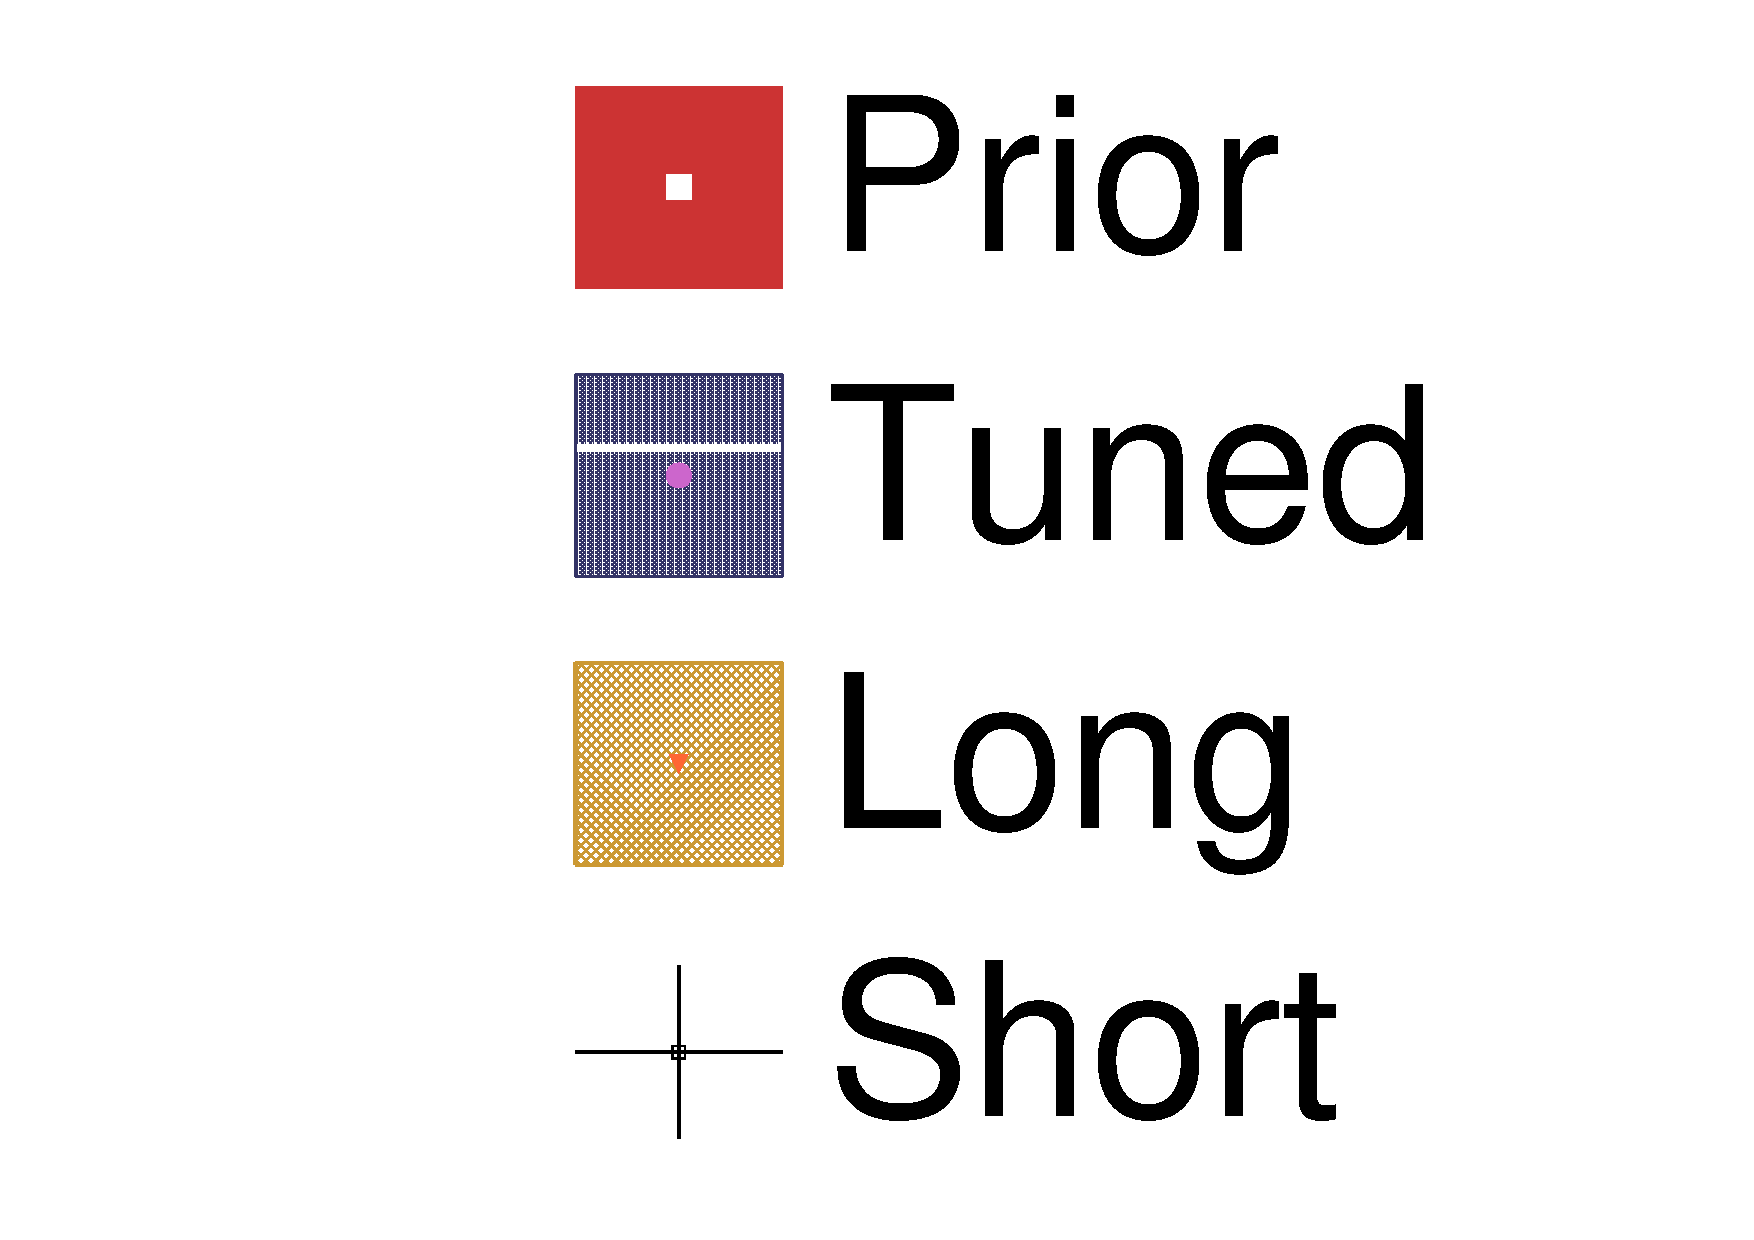
\includegraphics[width=\textwidth, trim={0mm 150mm 50mm 0mm}, clip,page=1]{figures/mach3/data/2017b_NewData_NewDet_UpdXsecStep_2Xsec_4Det_5Flux_0_2017b_June_NewDet_merge_2017b_NewDet_June_Long_0}
	\end{subfigure}
\begin{subfigure}[t]{0.1\textwidth}
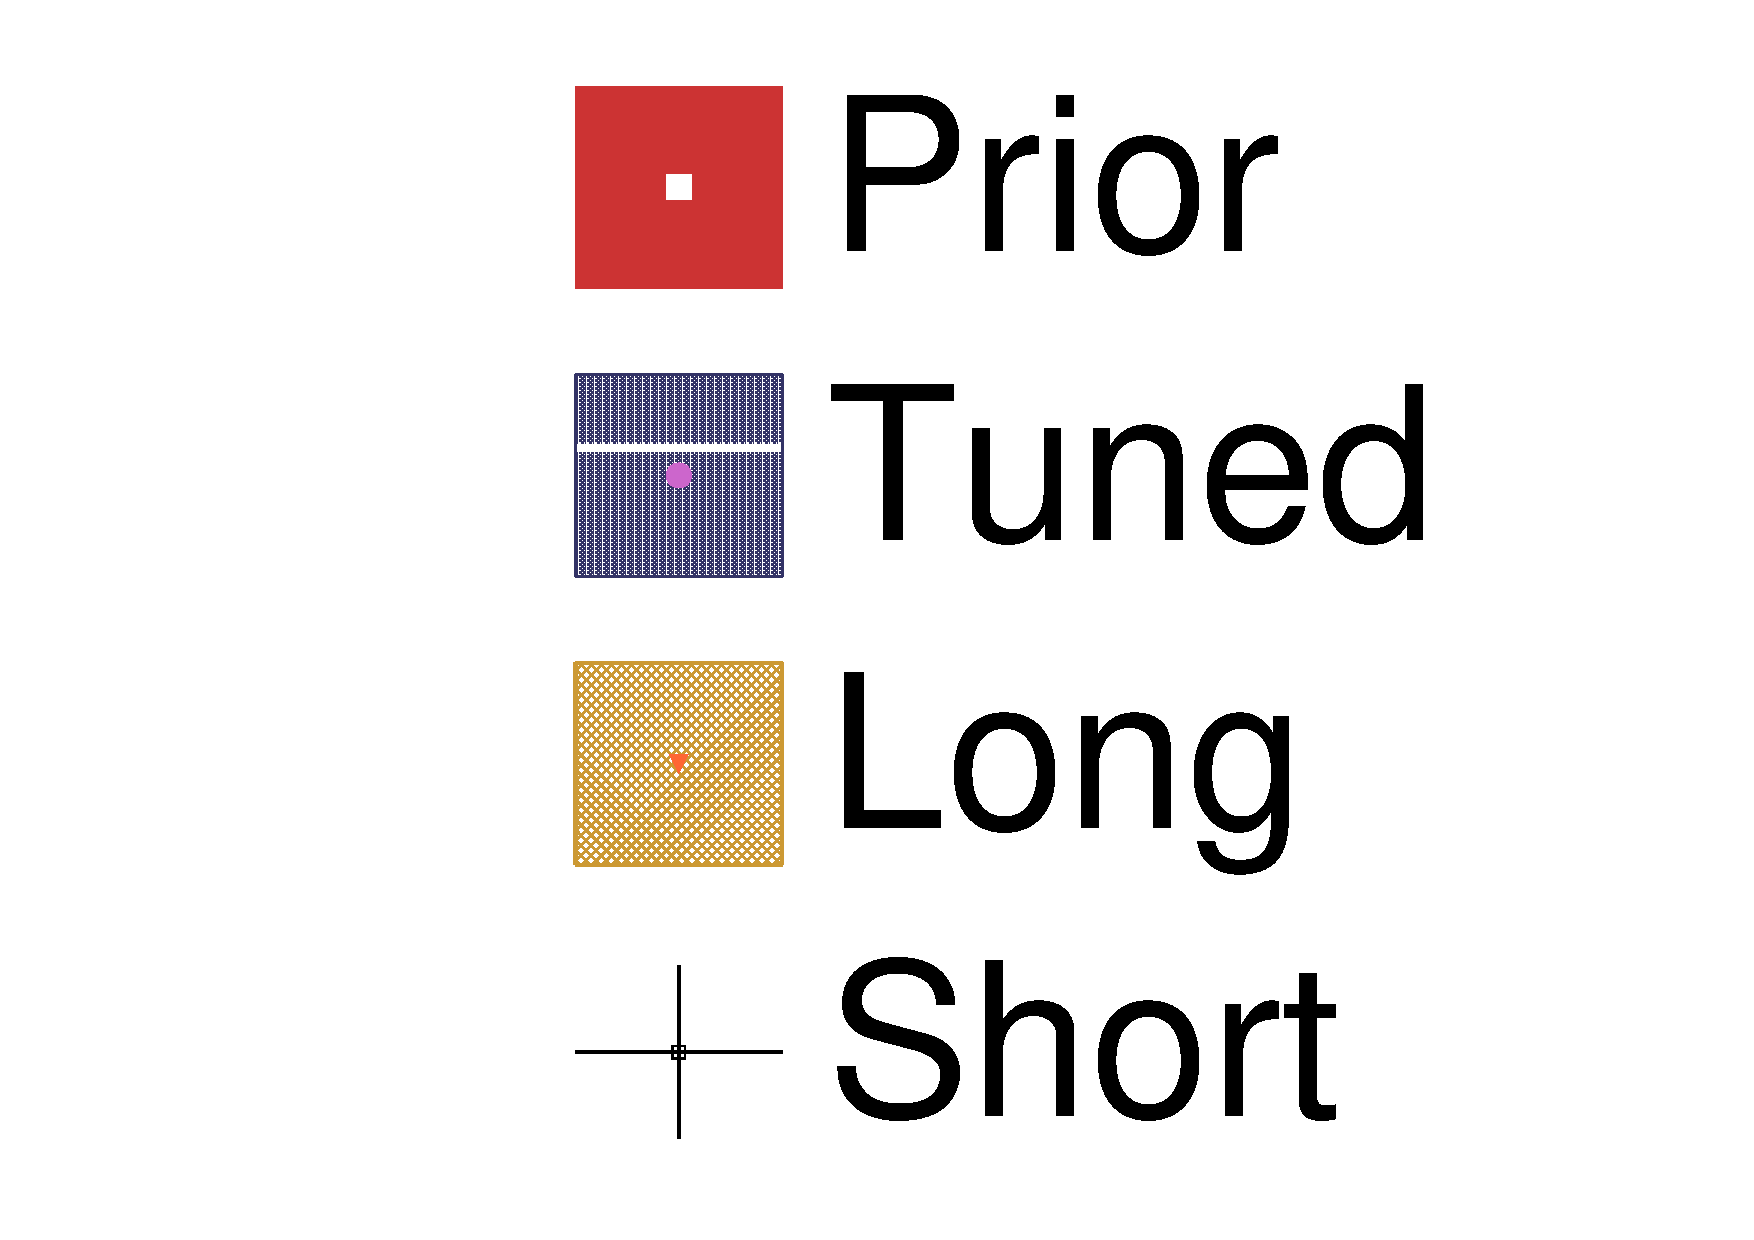
\includegraphics[width=\textwidth, trim={0mm 100mm 50mm 50mm}, clip,page=1]{figures/mach3/data/2017b_NewData_NewDet_UpdXsecStep_2Xsec_4Det_5Flux_0_2017b_June_NewDet_merge_2017b_NewDet_June_Long_0}
\end{subfigure}
\begin{subfigure}[t]{0.1\textwidth}
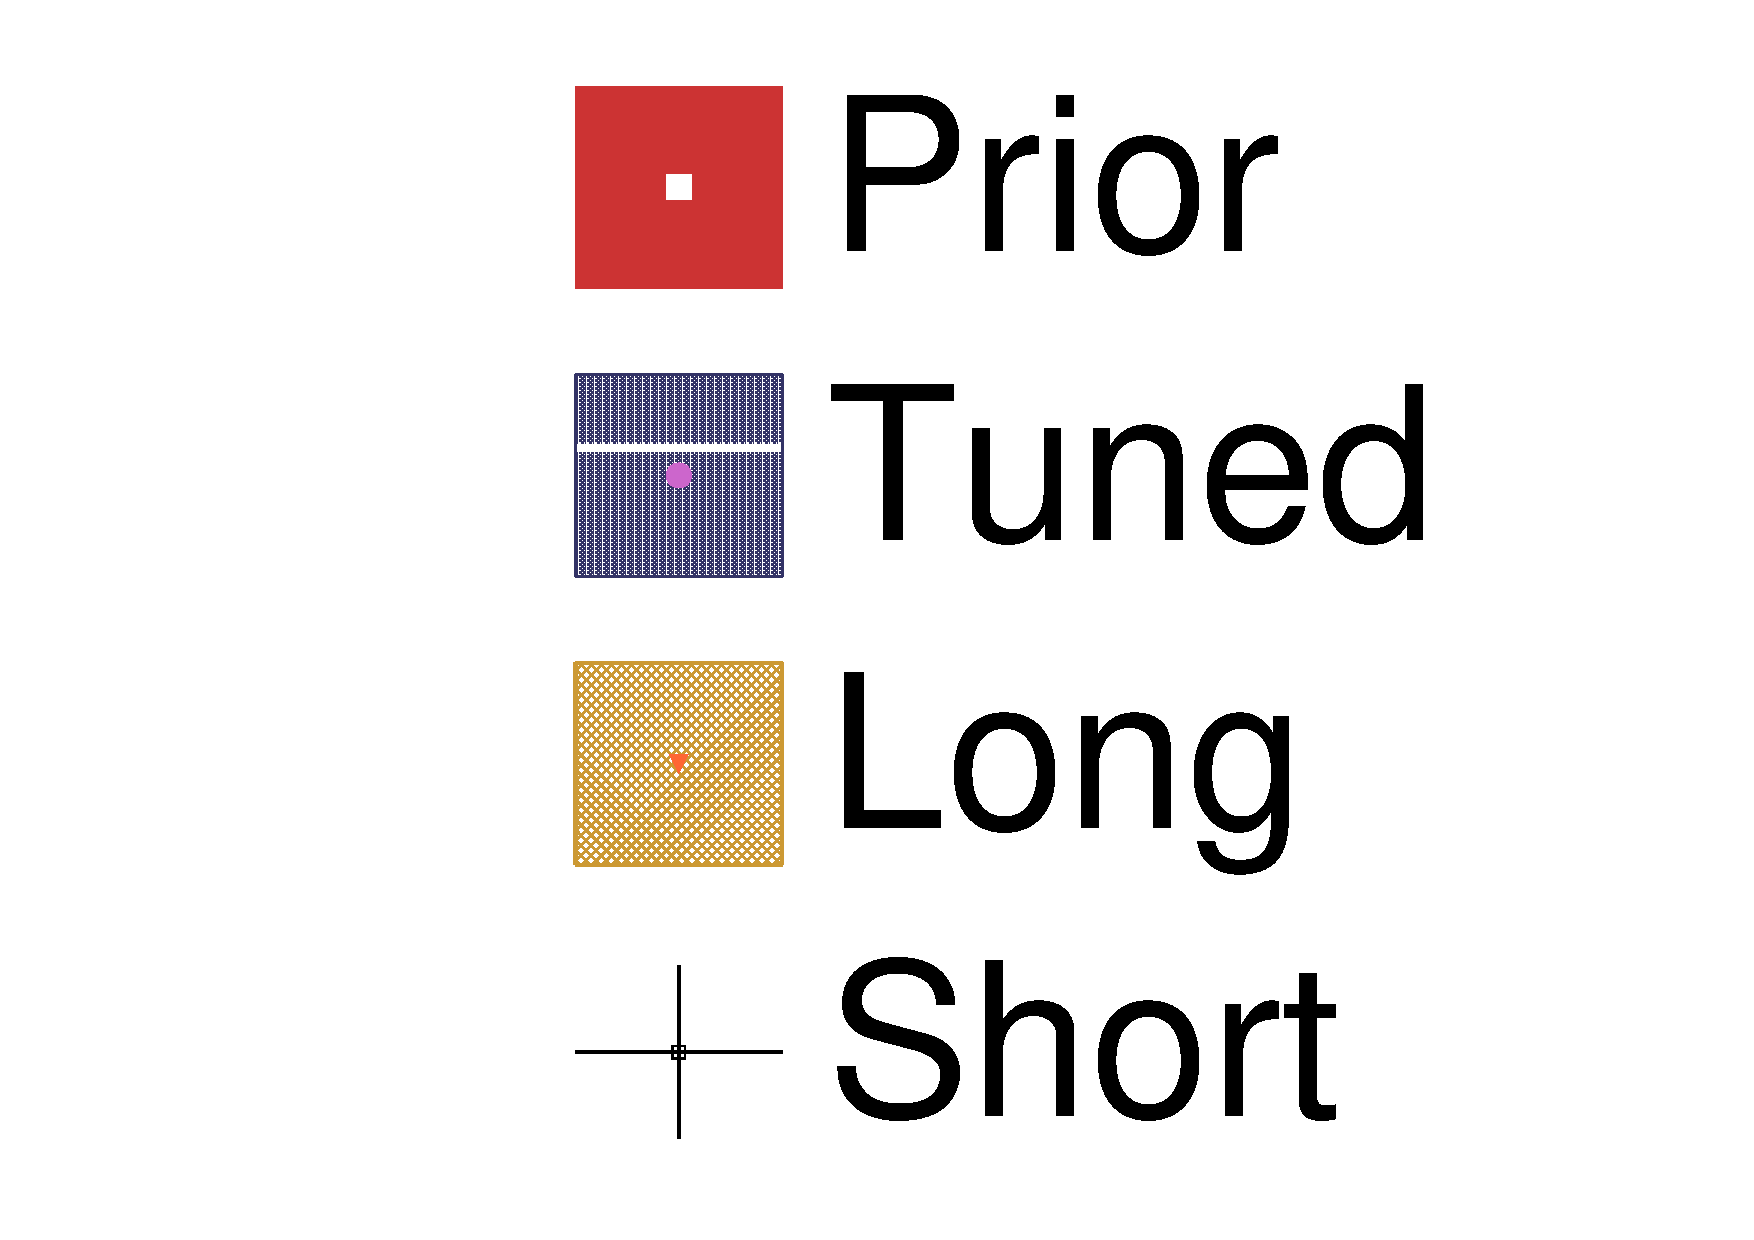
\includegraphics[width=\textwidth, trim={0mm 50mm 50mm 100mm}, clip,page=1]{figures/mach3/data/2017b_NewData_NewDet_UpdXsecStep_2Xsec_4Det_5Flux_0_2017b_June_NewDet_merge_2017b_NewDet_June_Long_0}
\end{subfigure}
\begin{subfigure}[t]{0.1\textwidth}
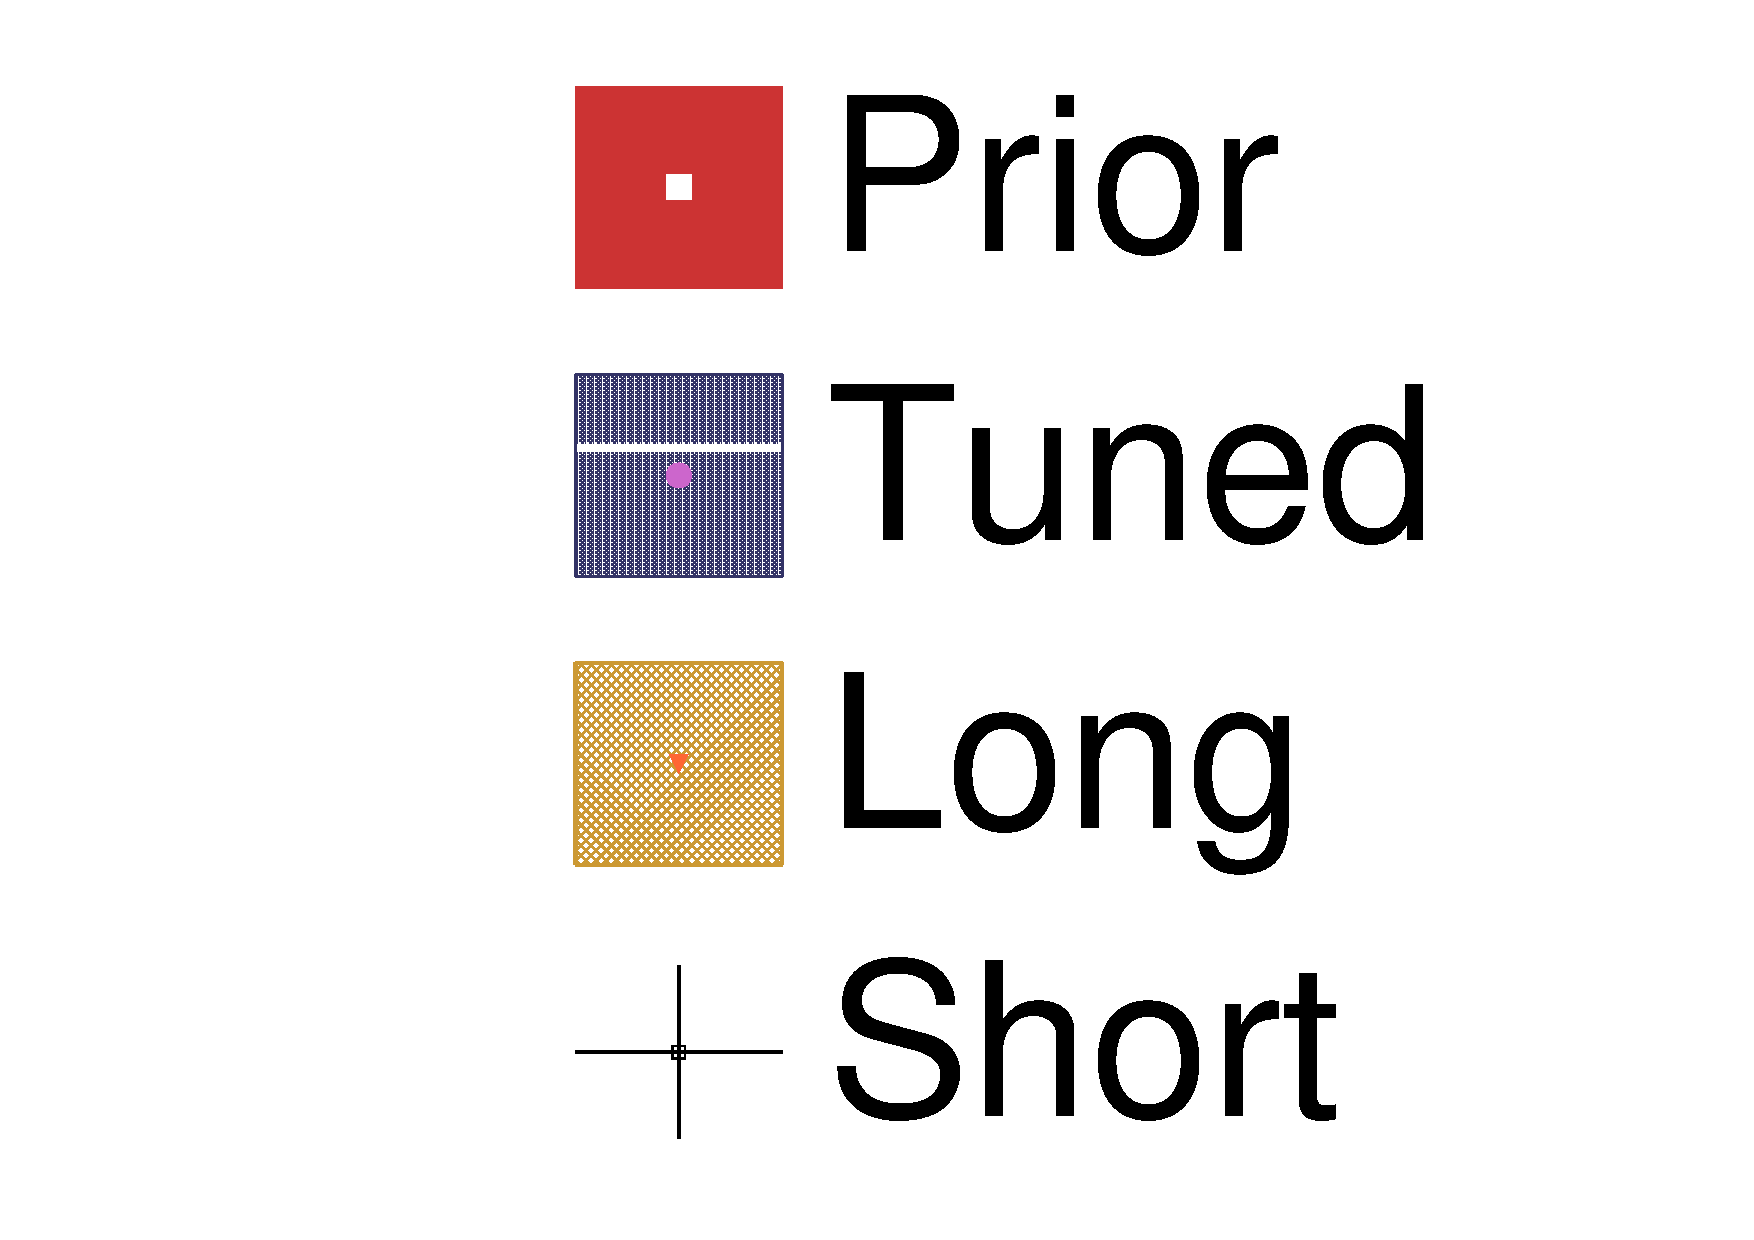
\includegraphics[width=\textwidth, trim={0mm 0mm 50mm 150mm}, clip,page=1]{figures/mach3/data/2017b_NewData_NewDet_UpdXsecStep_2Xsec_4Det_5Flux_0_2017b_June_NewDet_merge_2017b_NewDet_June_Long_0}
\end{subfigure}
	
	\begin{subfigure}[t]{0.24\textwidth}
		\includegraphics[width=\textwidth, trim={0mm 0mm 0mm 0mm}, clip,page=2]{figures/mach3/data/2017b_NewData_NewDet_UpdXsecStep_2Xsec_4Det_5Flux_0_2017b_June_NewDet_merge_2017b_NewDet_June_Long_0}
	\end{subfigure}
	\begin{subfigure}[t]{0.24\textwidth}
		\includegraphics[width=\textwidth, trim={0mm 0mm 0mm 0mm}, clip,page=3]{figures/mach3/data/2017b_NewData_NewDet_UpdXsecStep_2Xsec_4Det_5Flux_0_2017b_June_NewDet_merge_2017b_NewDet_June_Long_0}
	\end{subfigure}
	\begin{subfigure}[t]{0.24\textwidth}
		\includegraphics[width=\textwidth, trim={0mm 0mm 0mm 0mm}, clip,page=4]{figures/mach3/data/2017b_NewData_NewDet_UpdXsecStep_2Xsec_4Det_5Flux_0_2017b_June_NewDet_merge_2017b_NewDet_June_Long_0}
	\end{subfigure}
	\begin{subfigure}[t]{0.24\textwidth}
		\includegraphics[width=\textwidth, trim={0mm 0mm 0mm 0mm}, clip,page=5]{figures/mach3/data/2017b_NewData_NewDet_UpdXsecStep_2Xsec_4Det_5Flux_0_2017b_June_NewDet_merge_2017b_NewDet_June_Long_0}
	\end{subfigure}
	
	\begin{subfigure}[t]{0.24\textwidth}
		\includegraphics[width=\textwidth, trim={0mm 0mm 0mm 0mm}, clip,page=10]{figures/mach3/data/2017b_NewData_NewDet_UpdXsecStep_2Xsec_4Det_5Flux_0_2017b_June_NewDet_merge_2017b_NewDet_June_Long_0}
	\end{subfigure}
	\begin{subfigure}[t]{0.24\textwidth}
		\includegraphics[width=\textwidth, trim={0mm 0mm 0mm 0mm}, clip,page=11]{figures/mach3/data/2017b_NewData_NewDet_UpdXsecStep_2Xsec_4Det_5Flux_0_2017b_June_NewDet_merge_2017b_NewDet_June_Long_0}
	\end{subfigure}
	\begin{subfigure}[t]{0.24\textwidth}
		\includegraphics[width=\textwidth, trim={0mm 0mm 0mm 0mm}, clip,page=12]{figures/mach3/data/2017b_NewData_NewDet_UpdXsecStep_2Xsec_4Det_5Flux_0_2017b_June_NewDet_merge_2017b_NewDet_June_Long_0}
	\end{subfigure}
	\begin{subfigure}[t]{0.24\textwidth}
		\includegraphics[width=\textwidth, trim={0mm 0mm 0mm 0mm}, clip,page=13]{figures/mach3/data/2017b_NewData_NewDet_UpdXsecStep_2Xsec_4Det_5Flux_0_2017b_June_NewDet_merge_2017b_NewDet_June_Long_0}
	\end{subfigure}
	\caption{FHC flux parameters after the data fit for different MCMC chains}
	\label{fig:flux_data_fhc}
\end{figure}

\autoref{fig:flux_data_rhc} shows the RHC flux parameters post-fit. There is a decrease of \numubar for low energies to approximately 0.96, which increases to the nominal at $E_\nu=0.6\text{ GeV}$. At higher energies the normalisations go back to around 0.96. The only increase observed are the \nuebar parameters around 0.6 GeV. No parameters leave the 1$\sigma$ prior.
\begin{figure}[h]	
	\begin{subfigure}[t]{0.1\textwidth}
		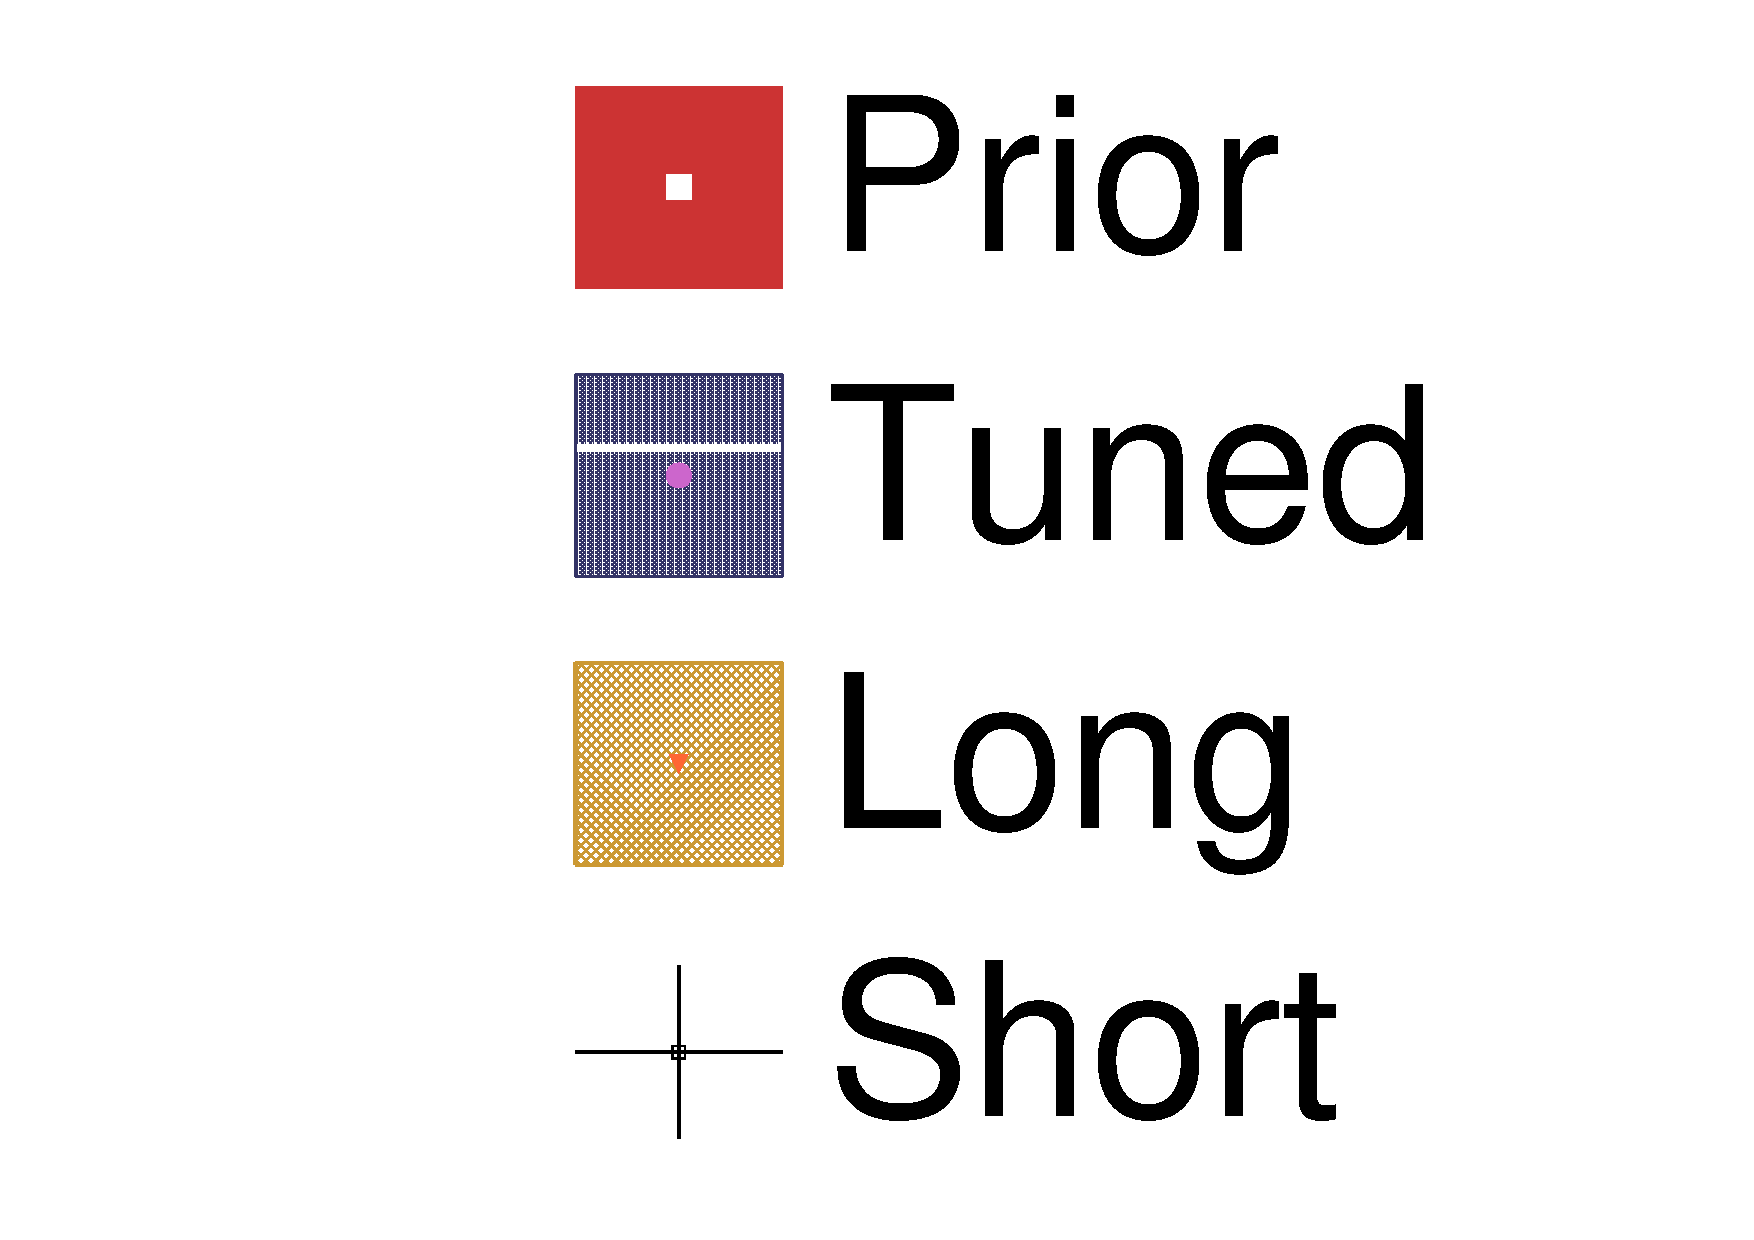
\includegraphics[width=\textwidth, trim={0mm 150mm 50mm 0mm}, clip,page=1]{figures/mach3/data/2017b_NewData_NewDet_UpdXsecStep_2Xsec_4Det_5Flux_0_2017b_June_NewDet_merge_2017b_NewDet_June_Long_0}
	\end{subfigure}
	\begin{subfigure}[t]{0.1\textwidth}
		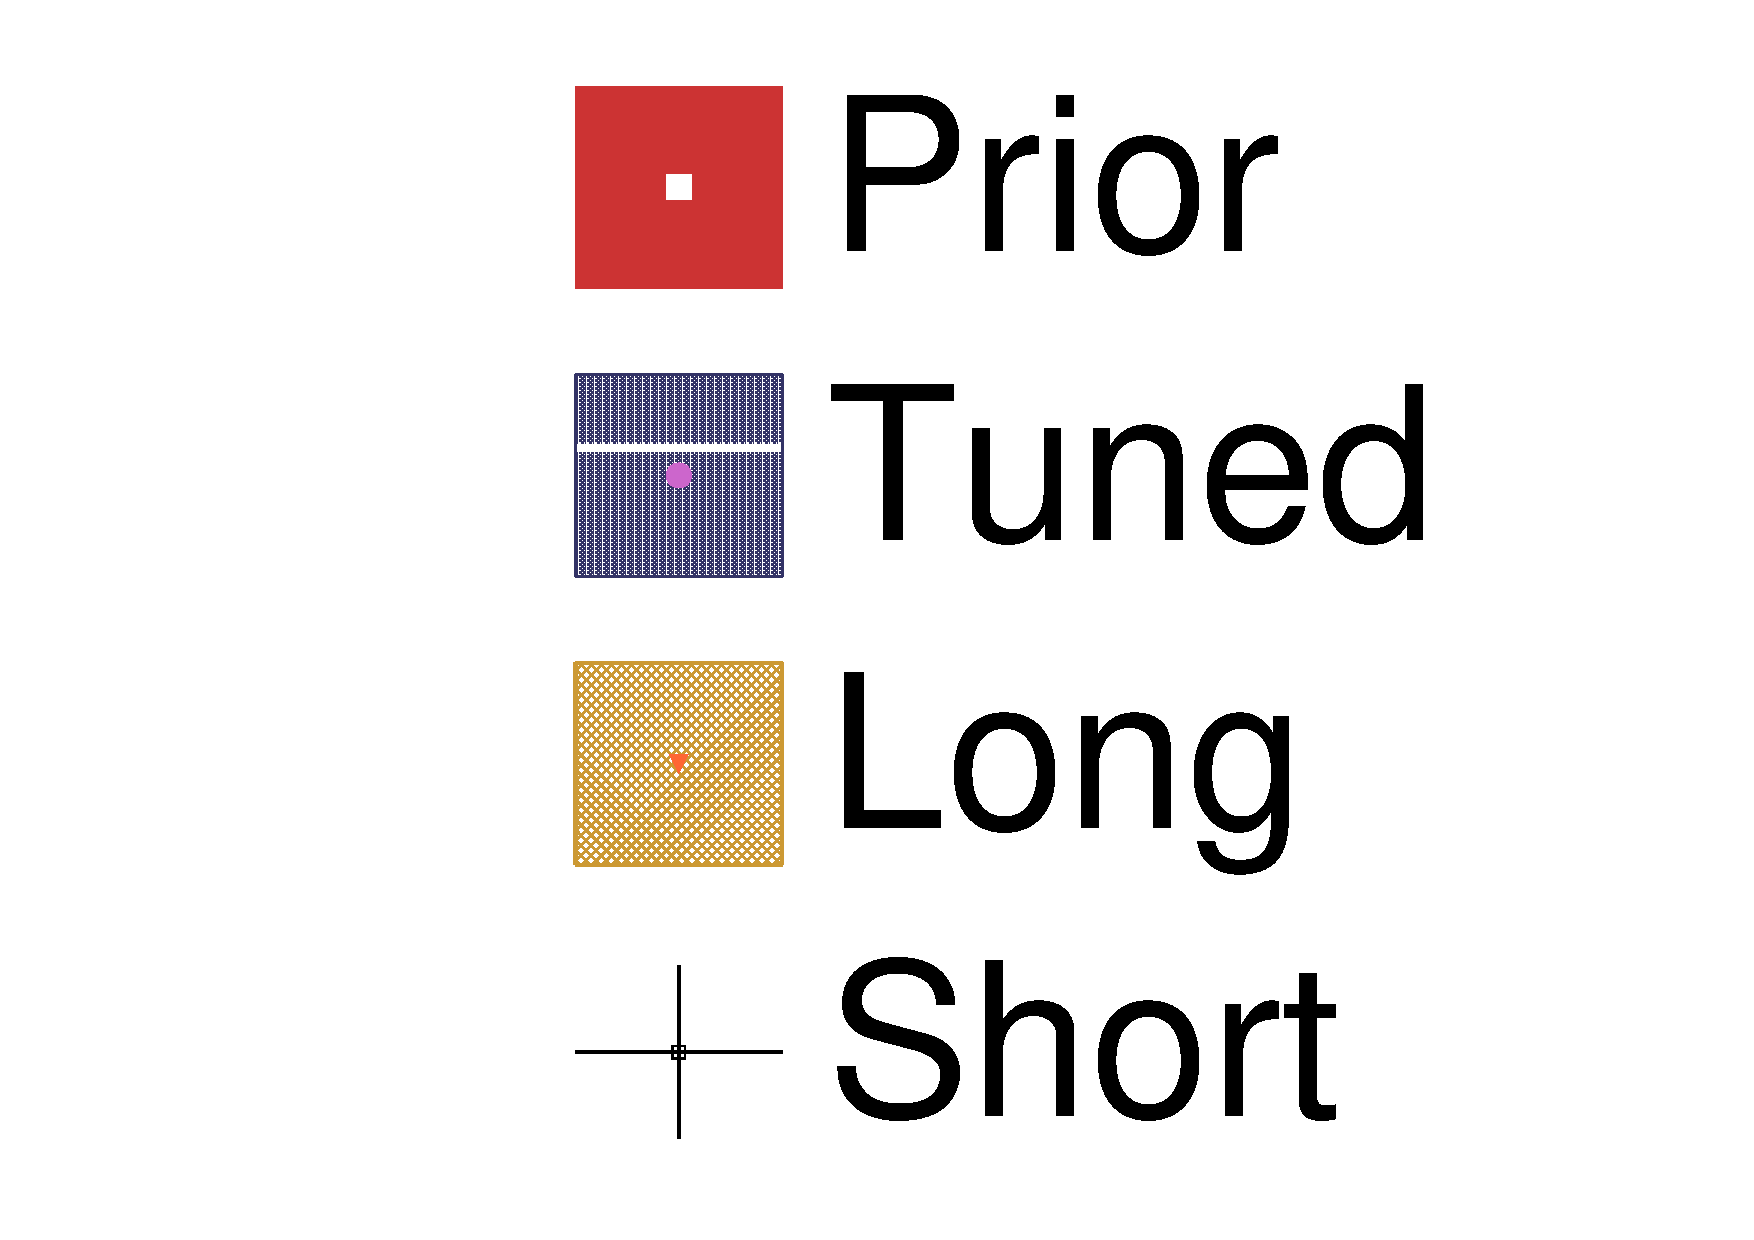
\includegraphics[width=\textwidth, trim={0mm 100mm 50mm 50mm}, clip,page=1]{figures/mach3/data/2017b_NewData_NewDet_UpdXsecStep_2Xsec_4Det_5Flux_0_2017b_June_NewDet_merge_2017b_NewDet_June_Long_0}
	\end{subfigure}
	\begin{subfigure}[t]{0.1\textwidth}
		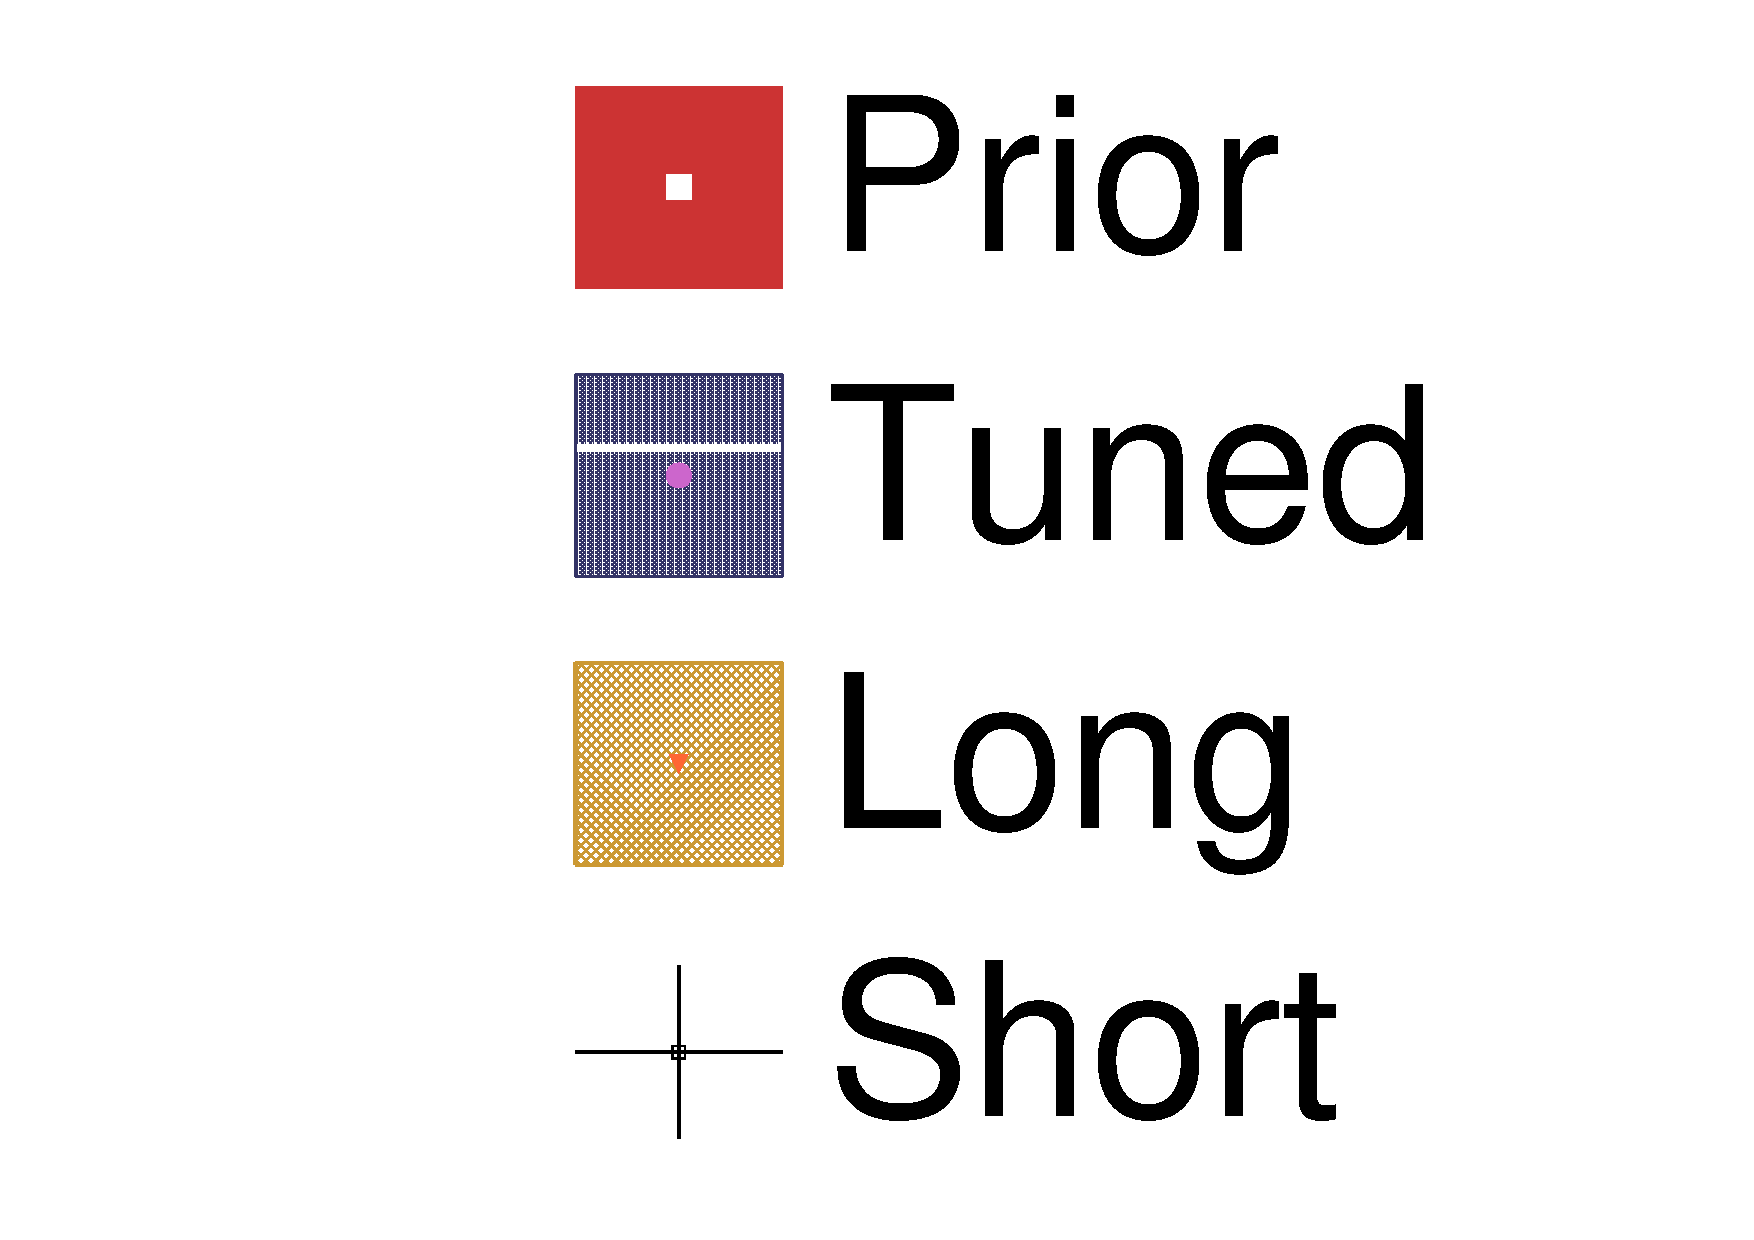
\includegraphics[width=\textwidth, trim={0mm 50mm 50mm 100mm}, clip,page=1]{figures/mach3/data/2017b_NewData_NewDet_UpdXsecStep_2Xsec_4Det_5Flux_0_2017b_June_NewDet_merge_2017b_NewDet_June_Long_0}
	\end{subfigure}
	\begin{subfigure}[t]{0.1\textwidth}
		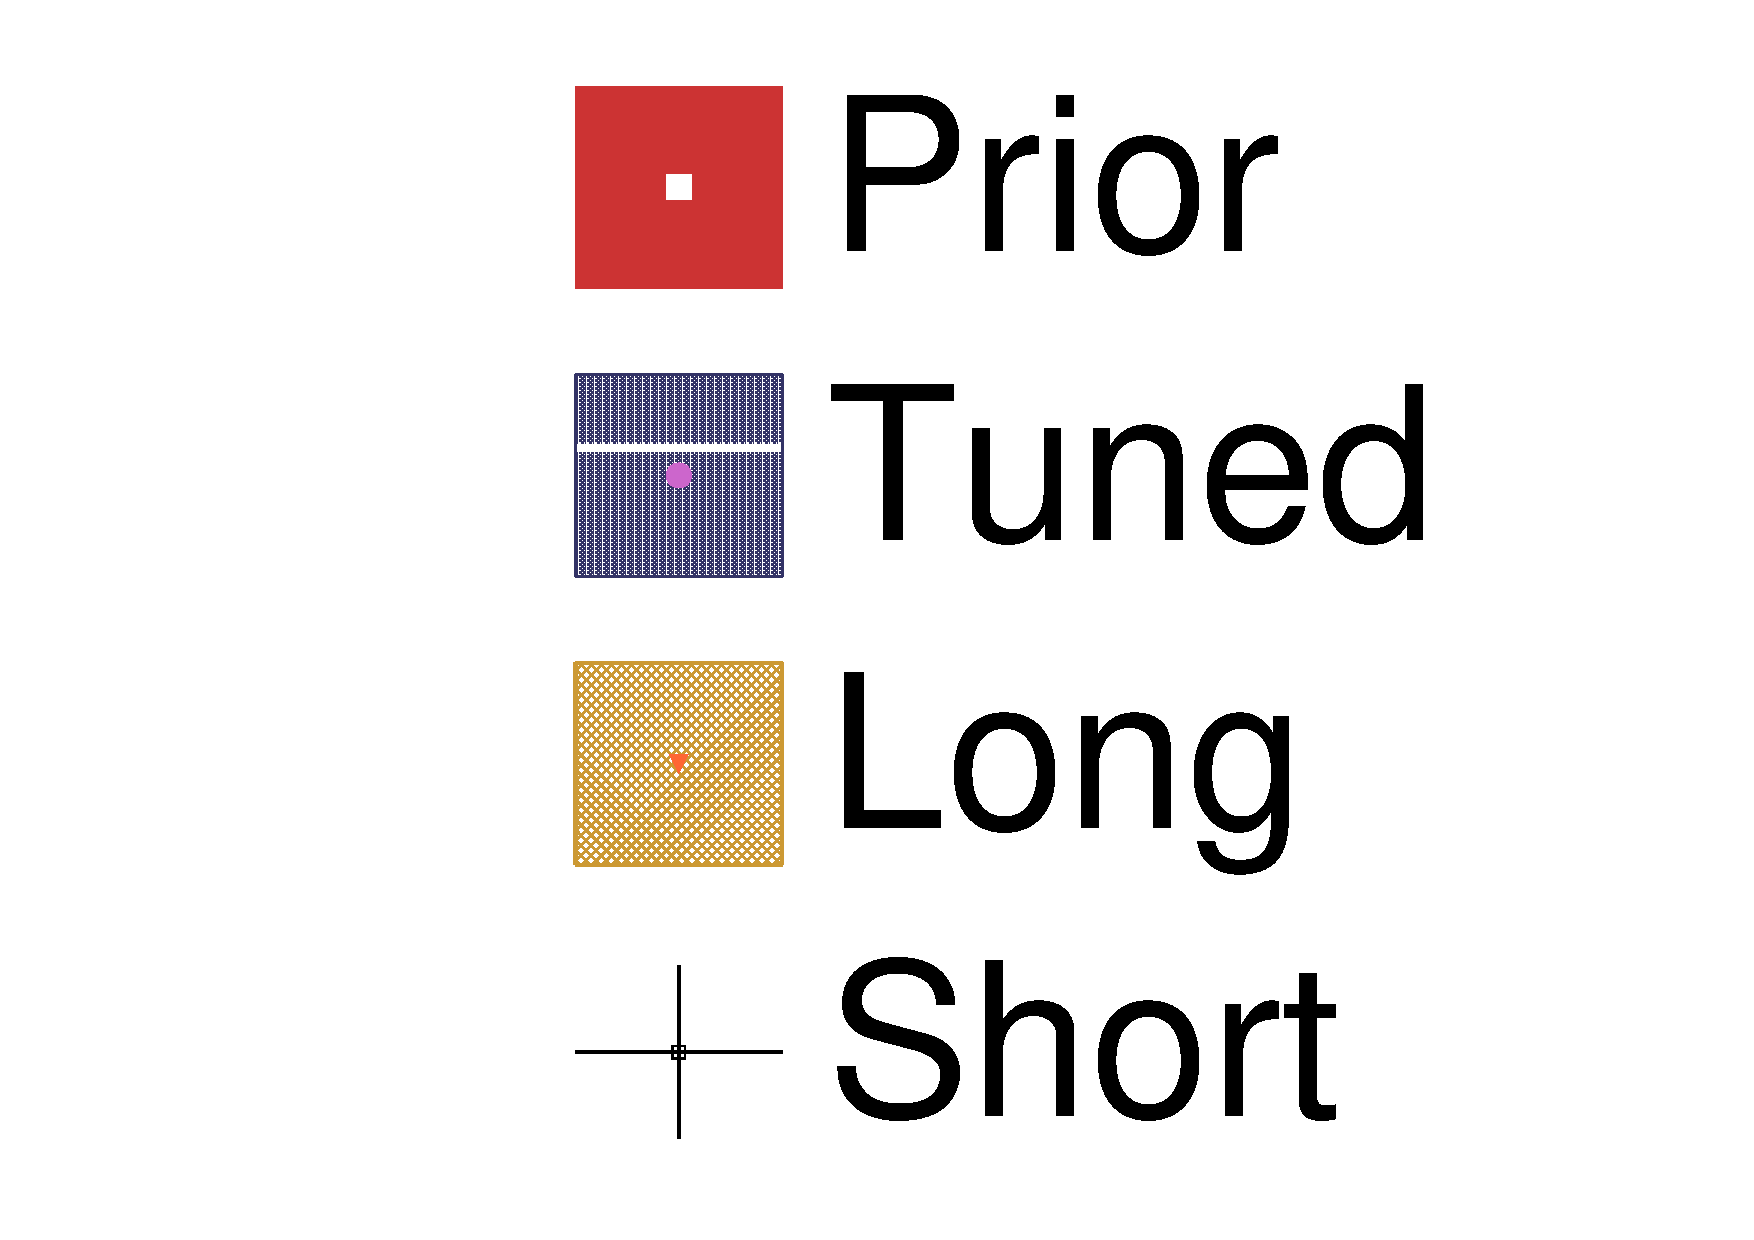
\includegraphics[width=\textwidth, trim={0mm 0mm 50mm 150mm}, clip,page=1]{figures/mach3/data/2017b_NewData_NewDet_UpdXsecStep_2Xsec_4Det_5Flux_0_2017b_June_NewDet_merge_2017b_NewDet_June_Long_0}
	\end{subfigure}

	\begin{subfigure}[t]{0.24\textwidth}
		\includegraphics[width=\textwidth, trim={0mm 0mm 0mm 0mm}, clip,page=6]{figures/mach3/data/2017b_NewData_NewDet_UpdXsecStep_2Xsec_4Det_5Flux_0_2017b_June_NewDet_merge_2017b_NewDet_June_Long_0}
	\end{subfigure}
	\begin{subfigure}[t]{0.24\textwidth}
		\includegraphics[width=\textwidth, trim={0mm 0mm 0mm 0mm}, clip,page=7]{figures/mach3/data/2017b_NewData_NewDet_UpdXsecStep_2Xsec_4Det_5Flux_0_2017b_June_NewDet_merge_2017b_NewDet_June_Long_0}
	\end{subfigure}
	\begin{subfigure}[t]{0.24\textwidth}
		\includegraphics[width=\textwidth, trim={0mm 0mm 0mm 0mm}, clip,page=8]{figures/mach3/data/2017b_NewData_NewDet_UpdXsecStep_2Xsec_4Det_5Flux_0_2017b_June_NewDet_merge_2017b_NewDet_June_Long_0}
	\end{subfigure}
	\begin{subfigure}[t]{0.24\textwidth}
		\includegraphics[width=\textwidth, trim={0mm 0mm 0mm 0mm}, clip,page=9]{figures/mach3/data/2017b_NewData_NewDet_UpdXsecStep_2Xsec_4Det_5Flux_0_2017b_June_NewDet_merge_2017b_NewDet_June_Long_0}
	\end{subfigure}
	
	\begin{subfigure}[t]{0.24\textwidth}
		\includegraphics[width=\textwidth, trim={0mm 0mm 0mm 0mm}, clip,page=14]{figures/mach3/data/2017b_NewData_NewDet_UpdXsecStep_2Xsec_4Det_5Flux_0_2017b_June_NewDet_merge_2017b_NewDet_June_Long_0}
	\end{subfigure}
	\begin{subfigure}[t]{0.24\textwidth}
		\includegraphics[width=\textwidth, trim={0mm 0mm 0mm 0mm}, clip,page=15]{figures/mach3/data/2017b_NewData_NewDet_UpdXsecStep_2Xsec_4Det_5Flux_0_2017b_June_NewDet_merge_2017b_NewDet_June_Long_0}
	\end{subfigure}
	\begin{subfigure}[t]{0.24\textwidth}
		\includegraphics[width=\textwidth, trim={0mm 0mm 0mm 0mm}, clip,page=16]{figures/mach3/data/2017b_NewData_NewDet_UpdXsecStep_2Xsec_4Det_5Flux_0_2017b_June_NewDet_merge_2017b_NewDet_June_Long_0}
	\end{subfigure}
	\begin{subfigure}[t]{0.24\textwidth}
		\includegraphics[width=\textwidth, trim={0mm 0mm 0mm 0mm}, clip,page=17]{figures/mach3/data/2017b_NewData_NewDet_UpdXsecStep_2Xsec_4Det_5Flux_0_2017b_June_NewDet_merge_2017b_NewDet_June_Long_0}
	\end{subfigure}
	\caption{RHC flux parameters after the data fit for different MCMC chains}
	\label{fig:flux_data_rhc}
\end{figure}

\autoref{fig:xsec_data} show the interaction parameters after the fit, where we expect most of the parameter movement to happen. The largest deviations from the priors are seen for $M_A^{QE}$ and BeRPA B, followed by $M_A^{RES}$. 

The shift in $M_A^{QE}$ is expected since the ``prior'' central value is from tunes to nuclear data\cite{ccqe_tuning}. $M_A^{QE}$ is historically inflated\cite{k2k_ccqe_carbon,k2k_ccqe_oxygen,minos_ccqe_iron,miniboone_nu_ccqe} when not using adequate nuclear effects, such as RPA or 2p2h, which leads to it becoming an effective parameter instead. Using a flat prior on $M_A^{QE}$ leads toward values obtained from fits to nucleon data, $M_A^{QE}=1.069\pm0.016\text{ GeV}$ \cite{maqe_fit}. The post-fit value here in real units is $M_A^{QE}=1.12\pm0.07\text{ GeV}$.

The shifts in BeRPA are more worrisome. The low $Q^2$ parameters BeRPA A and BeRPA B are being pushed above their pre-fit $1\sigma$ uncertainties, indicating that the ND280 data has more events than the Monte-Carlo at low $Q^2$, possibly forcing a shape that isn't ``RPA-like''. \autoref{fig:berpa_data} shows the BeRPA weight being applied for every step in the data and Asimov chains: the nominal shape of the RPA correction is heavily distorted in the data fit, in which an increased cross-section at low $Q^2$ is strongly favoured. The weaker constraints above $Q^2=0.5\text{ GeV}^2$ reflect lacking data in the region.

The $M_A^{RES}$ parameter is pushed far from the bubble chamber tuned values (from $M_A^{RES}=1.07\pm0.15\text{ GeV}$ to $0.806\pm0.04\text{ GeV}$), whereas the other single pion production parameters are compatible with the prior. The may indicate sweeping up unmodelled nuclear effects (often approximately a function of $Q^2$) into the $M_A^{RES}$ parameter.

We note interesting 2p2h normalisations, in which the $\nu$ normalisation is 1.6, whereas $\bar{\nu}$ normalisation is 0.8, indicating some $\nu$ vs $\bar{\nu}$ tension in the nominal 2p2h model. The 2p2h shape parameters are pushed against their upper boundary, preferring a ``delta-like'' $q_0-q_3$ phase space, again indicating the 2p2h model does not agree with ND280 data.
\begin{figure}[h]
	\begin{subfigure}[t]{0.1\textwidth}
		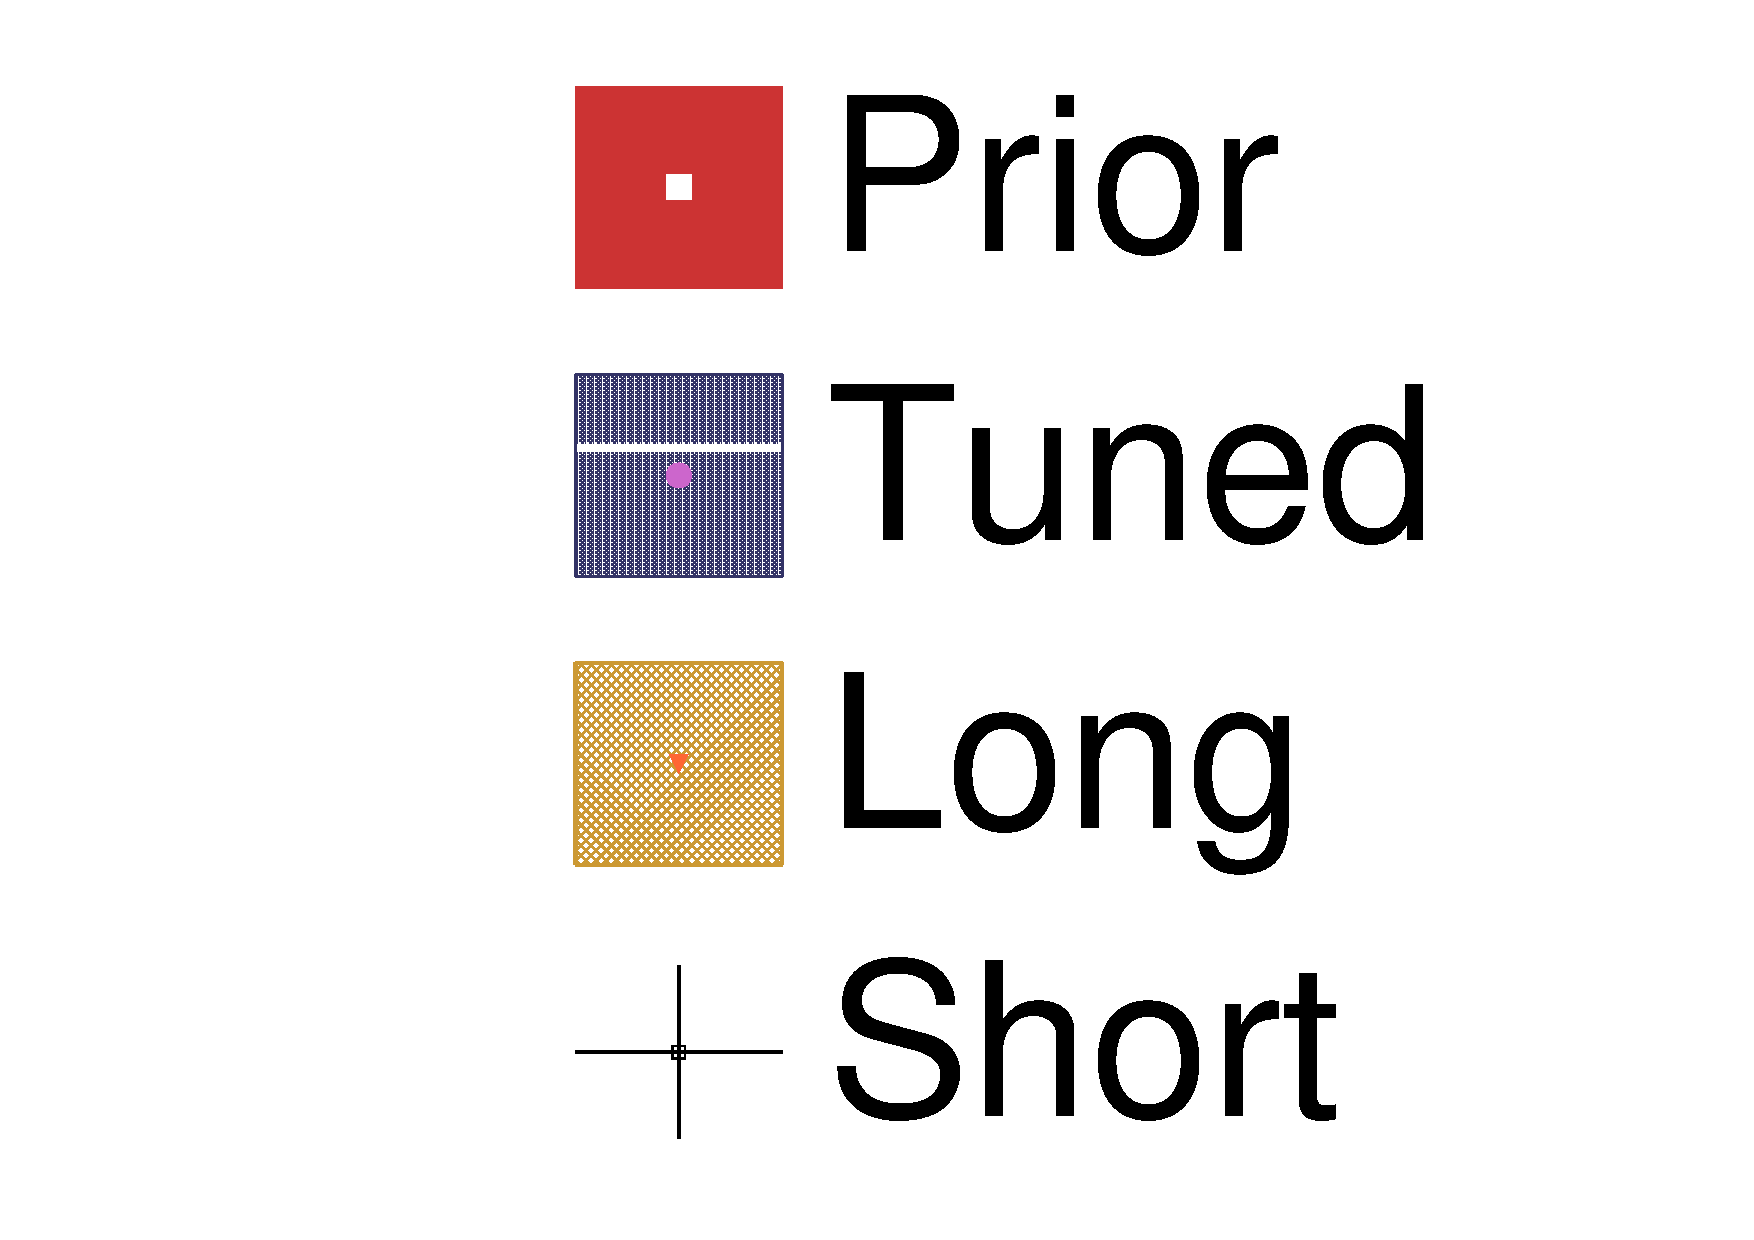
\includegraphics[width=\textwidth, trim={0mm 150mm 50mm 0mm}, clip,page=1]{figures/mach3/data/2017b_NewData_NewDet_UpdXsecStep_2Xsec_4Det_5Flux_0_2017b_June_NewDet_merge_2017b_NewDet_June_Long_0}
	\end{subfigure}
	\begin{subfigure}[t]{0.1\textwidth}
		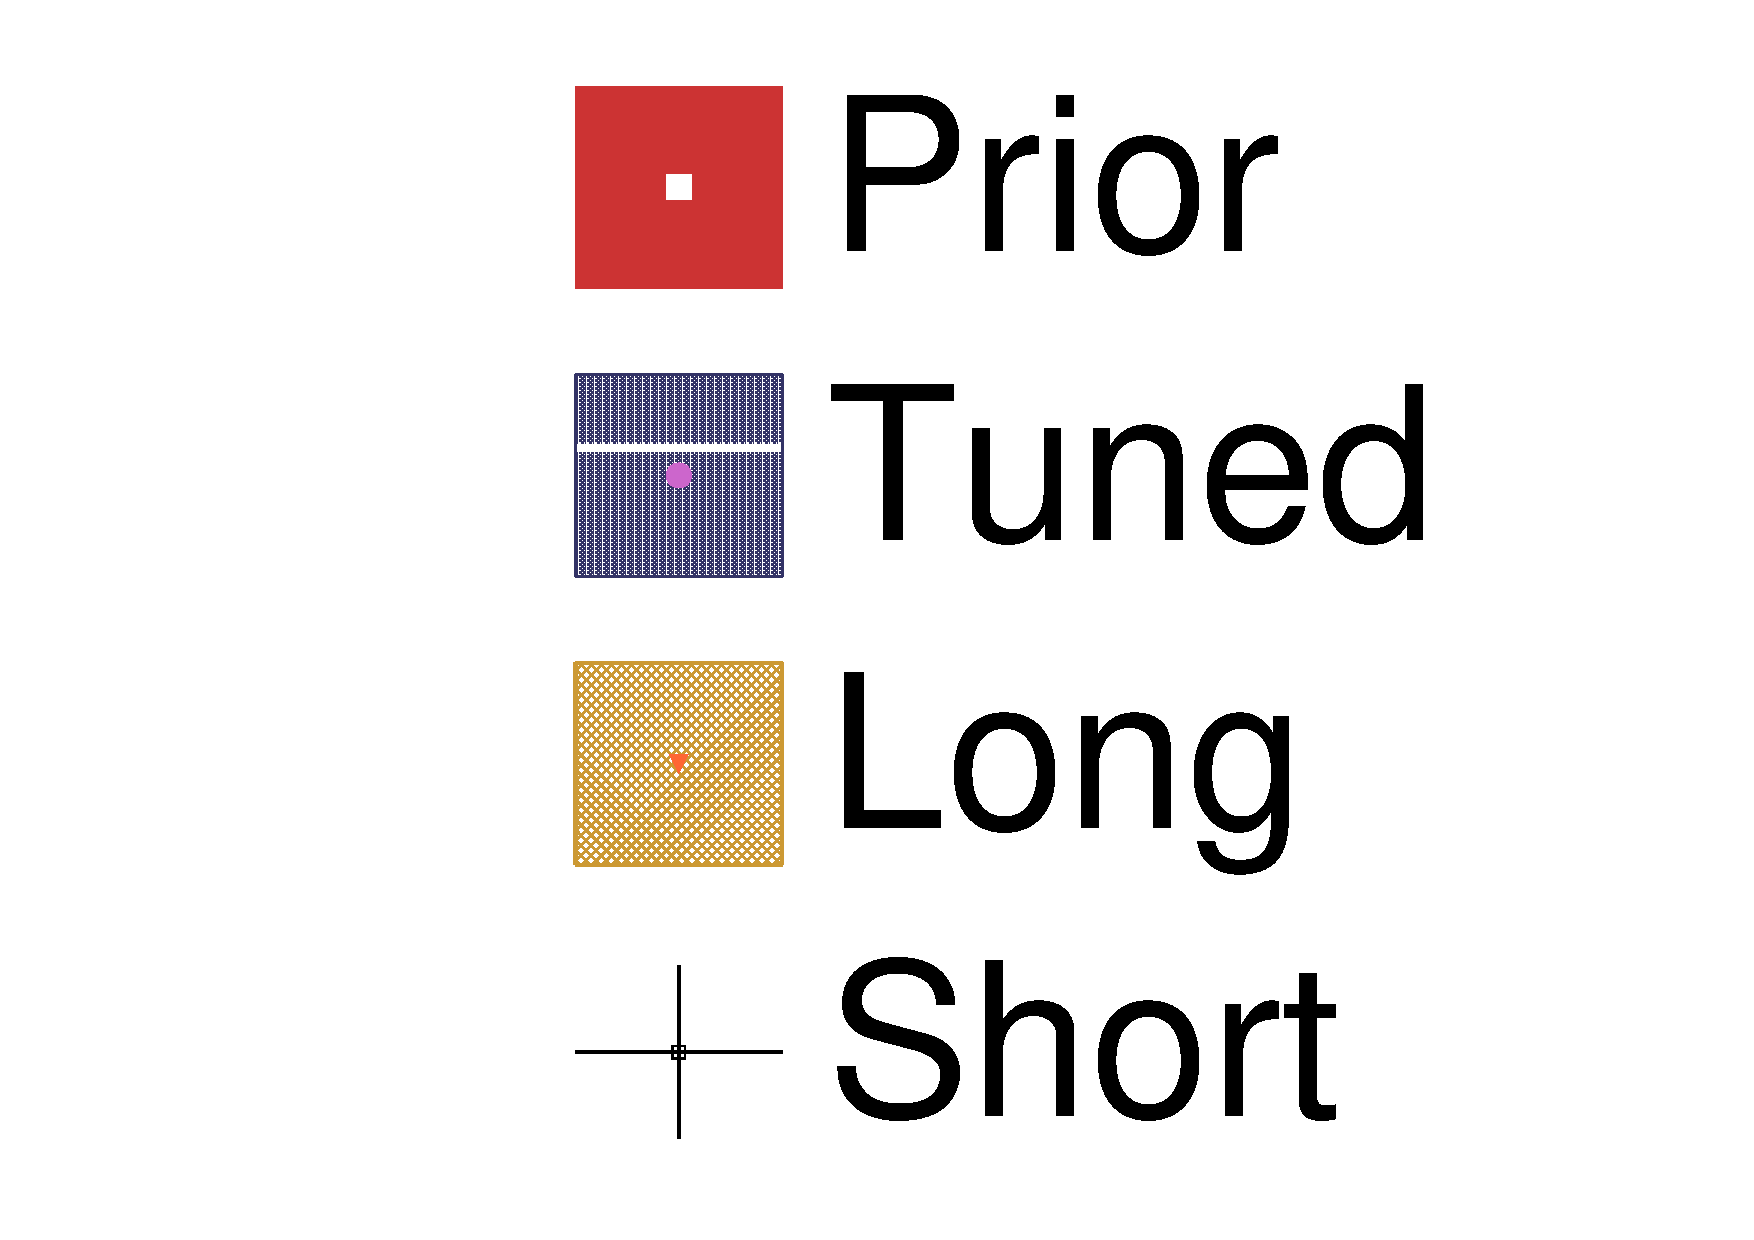
\includegraphics[width=\textwidth, trim={0mm 100mm 50mm 50mm}, clip,page=1]{figures/mach3/data/2017b_NewData_NewDet_UpdXsecStep_2Xsec_4Det_5Flux_0_2017b_June_NewDet_merge_2017b_NewDet_June_Long_0}
	\end{subfigure}
	\begin{subfigure}[t]{0.1\textwidth}
		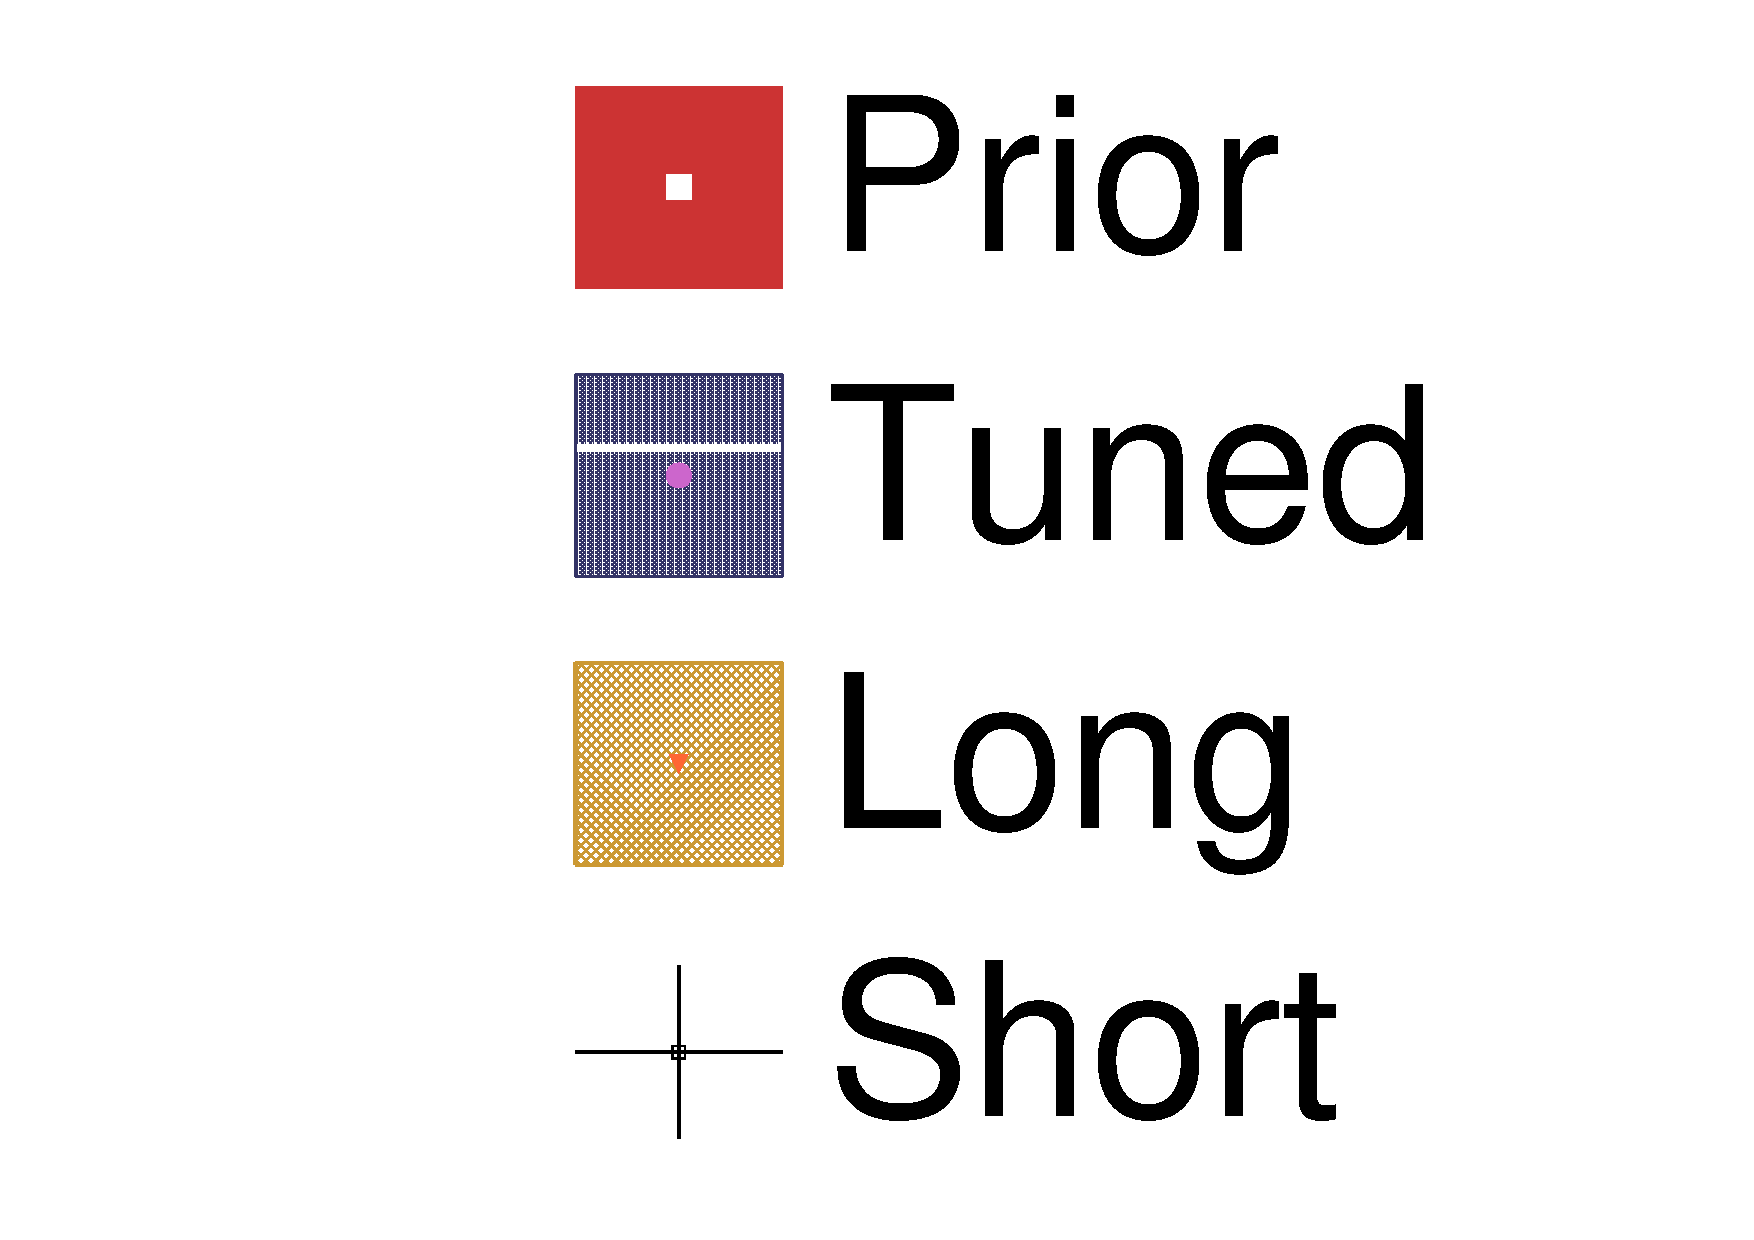
\includegraphics[width=\textwidth, trim={0mm 50mm 50mm 100mm}, clip,page=1]{figures/mach3/data/2017b_NewData_NewDet_UpdXsecStep_2Xsec_4Det_5Flux_0_2017b_June_NewDet_merge_2017b_NewDet_June_Long_0}
	\end{subfigure}
	\begin{subfigure}[t]{0.1\textwidth}
		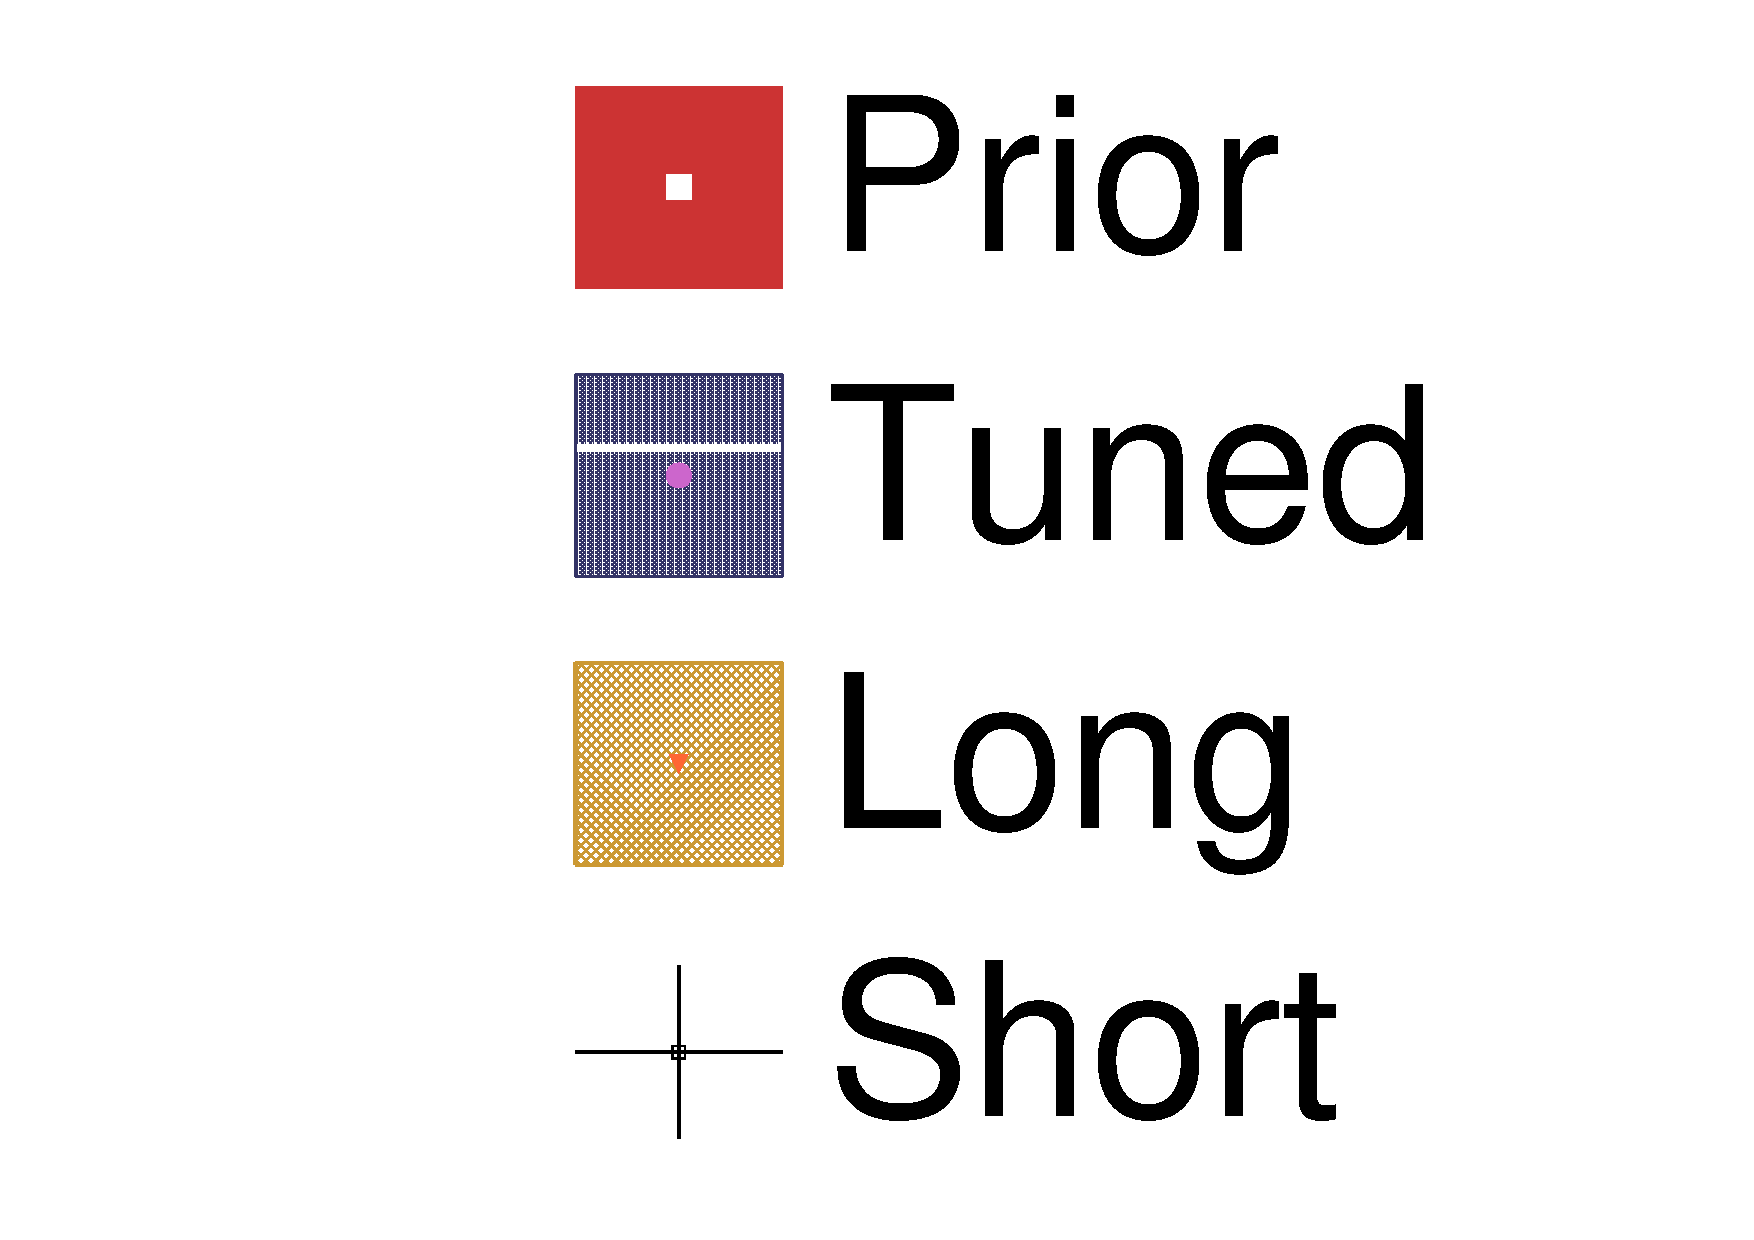
\includegraphics[width=\textwidth, trim={0mm 0mm 50mm 150mm}, clip,page=1]{figures/mach3/data/2017b_NewData_NewDet_UpdXsecStep_2Xsec_4Det_5Flux_0_2017b_June_NewDet_merge_2017b_NewDet_June_Long_0}
	\end{subfigure}

	\begin{subfigure}[t]{0.49\textwidth}
		\includegraphics[width=\textwidth, trim={0mm 0mm 0mm 0mm}, clip,page=18]{figures/mach3/data/2017b_NewData_NewDet_UpdXsecStep_2Xsec_4Det_5Flux_0_2017b_June_NewDet_merge_2017b_NewDet_June_Long_0}
	\end{subfigure}
	\begin{subfigure}[t]{0.49\textwidth}
		\includegraphics[width=\textwidth, trim={0mm 0mm 0mm 0mm}, clip,page=19]{figures/mach3/data/2017b_NewData_NewDet_UpdXsecStep_2Xsec_4Det_5Flux_0_2017b_June_NewDet_merge_2017b_NewDet_June_Long_0}
	\end{subfigure}
	
	\begin{subfigure}[t]{0.49\textwidth}
		\includegraphics[width=\textwidth, trim={0mm 0mm 0mm 0mm}, clip,page=20]{figures/mach3/data/2017b_NewData_NewDet_UpdXsecStep_2Xsec_4Det_5Flux_0_2017b_June_NewDet_merge_2017b_NewDet_June_Long_0}
	\end{subfigure}
	\begin{subfigure}[t]{0.49\textwidth}
		\includegraphics[width=\textwidth, trim={0mm 0mm 0mm 0mm}, clip,page=21]{figures/mach3/data/2017b_NewData_NewDet_UpdXsecStep_2Xsec_4Det_5Flux_0_2017b_June_NewDet_merge_2017b_NewDet_June_Long_0}
	\end{subfigure}
	\caption{Interaction parameters after the data fit for different MCMC chains}
	\label{fig:xsec_data}
\end{figure}

\begin{figure}[h]
	\begin{subfigure}[t]{0.49\textwidth}
		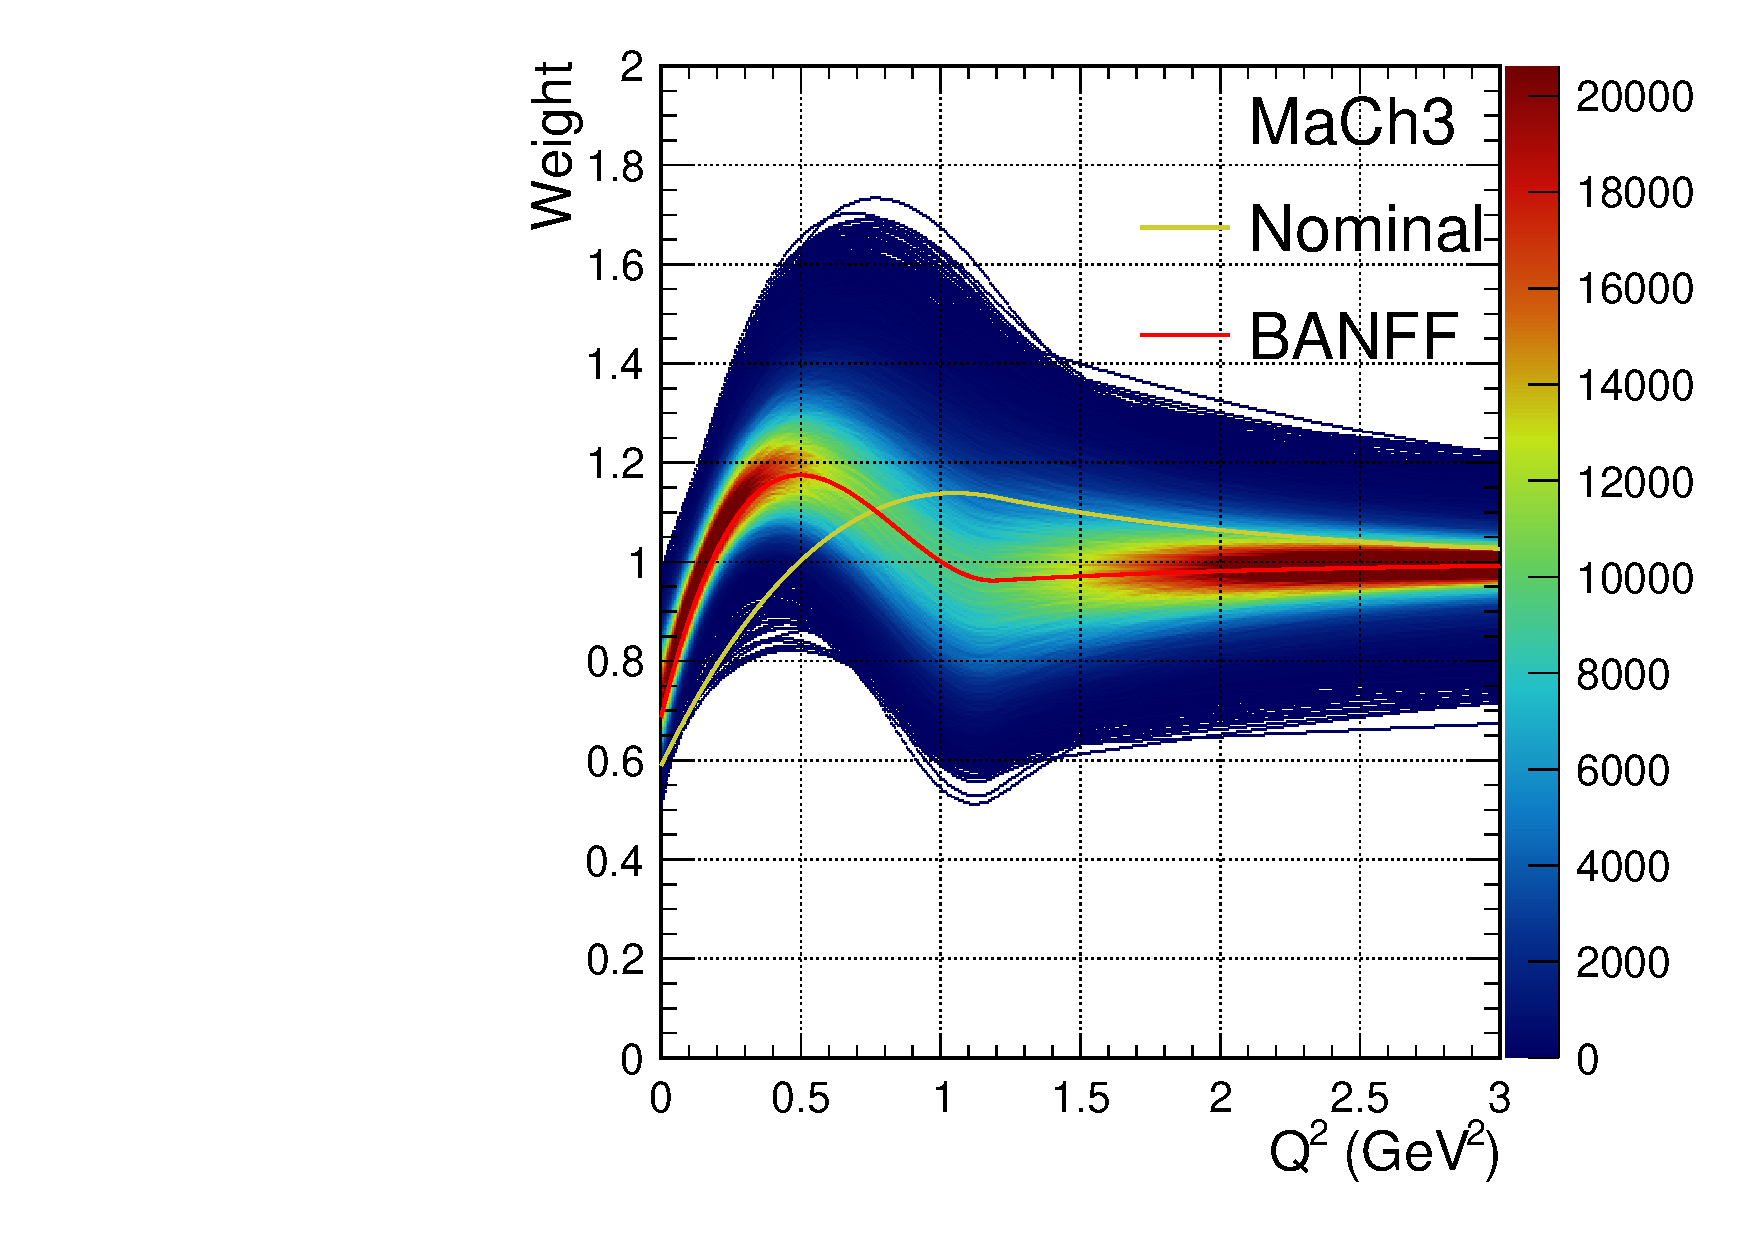
\includegraphics[width=\textwidth, trim={0mm 0mm 0mm 0mm}, clip,page=1]{figures/mach3/data/2017b_NewDet_3Xsec_4Det_5Flux_NewXSecTune_Data_0_BeRPA}
		\caption{BeRPA shape after fitting to data}
	\end{subfigure}
	\begin{subfigure}[t]{0.49\textwidth}
		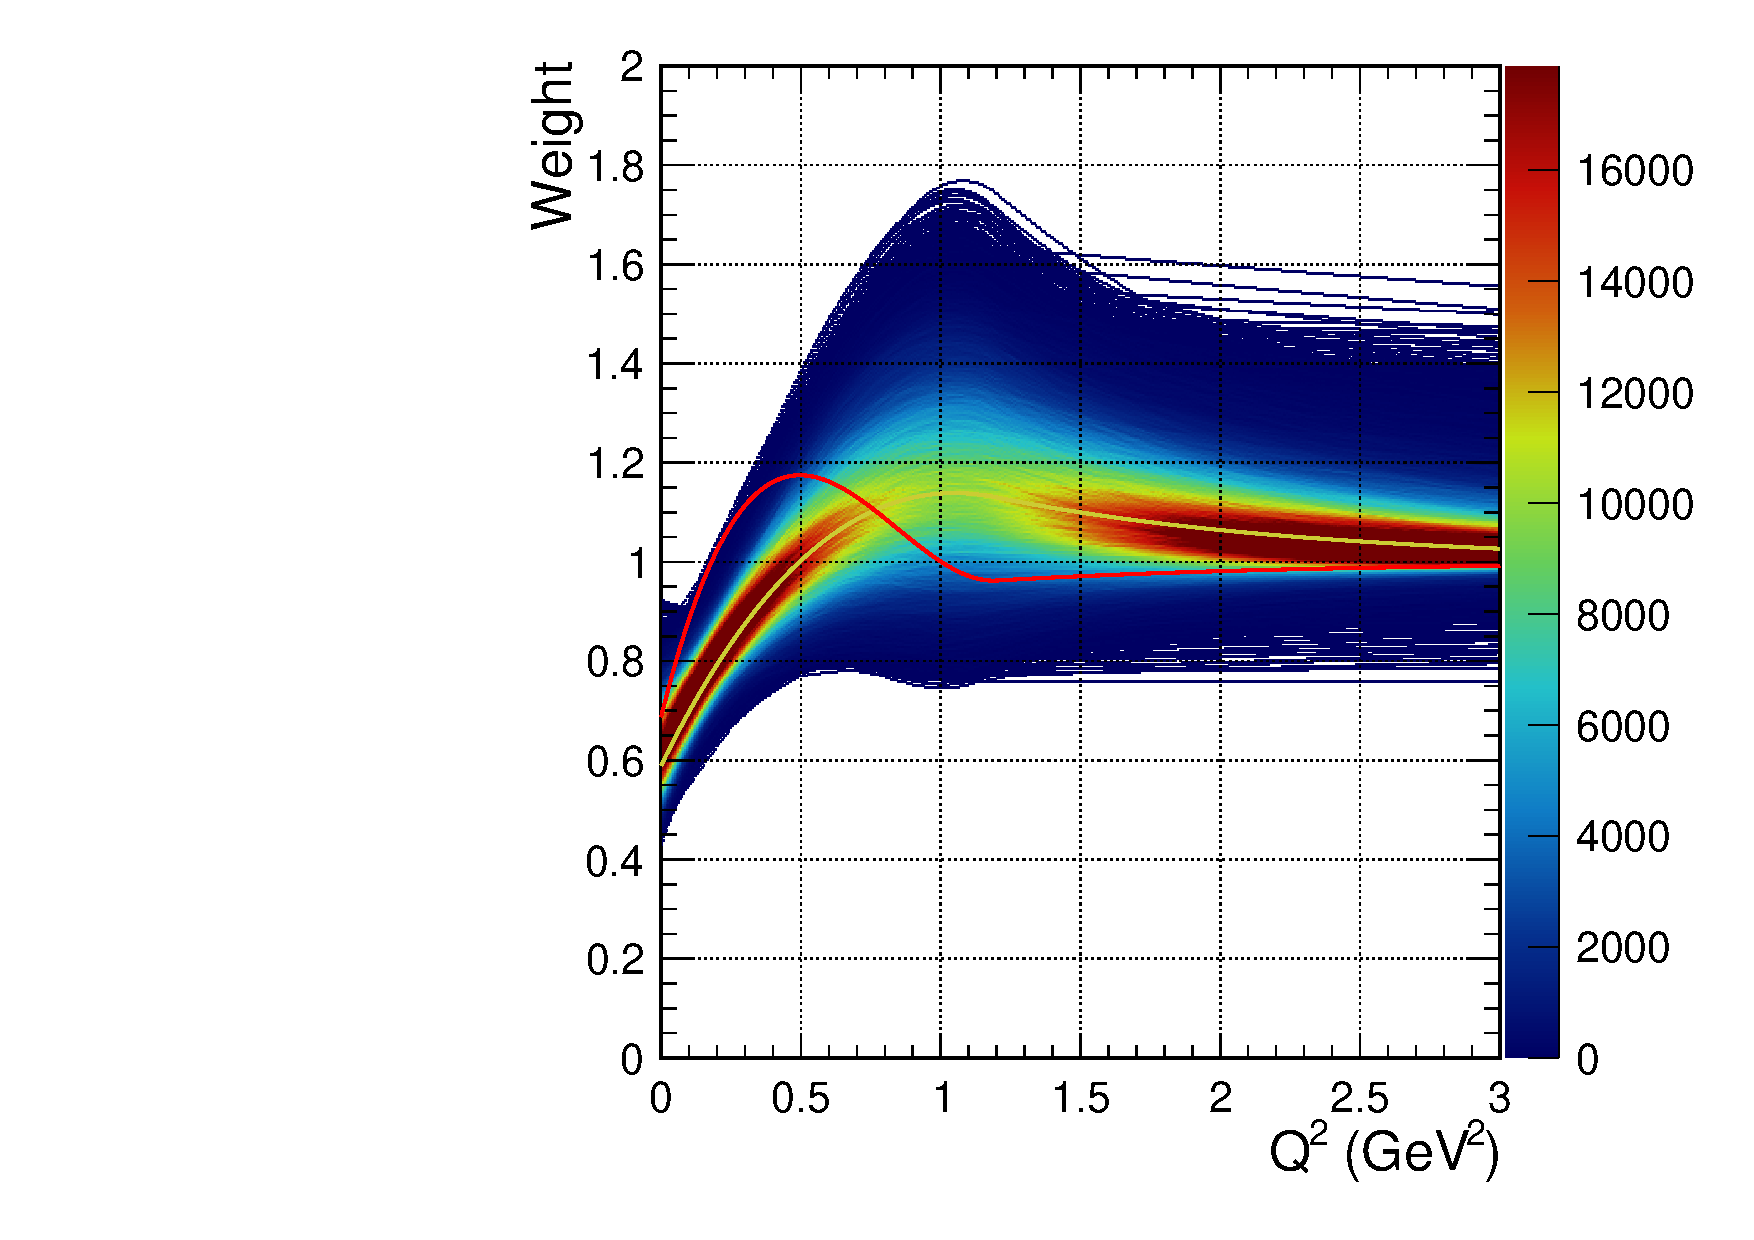
\includegraphics[width=\textwidth, trim={0mm 0mm 0mm 0mm}, clip,page=1]{figures/mach3/data/2017b_NewDet_3Xsec_4Det_5Flux_NewXSecTune_Asimov_0_BeRPA}
		\caption{BeRPA shape after fitting to Asimov}
	\end{subfigure}
\caption{BeRPA shape for each MCMC step for the tuned fits to data and Asimov}
\label{fig:berpa_data}
\end{figure}

To understand why BeRPA is heavily distorted from the nominal form, we look at the reconstructed $Q^2$ distributions of the CC0$\pi$ selections in \autoref{fig:fgd1_cc0pi_q2_berpa} and \autoref{fig:fgd2_cc0pi_q2_berpa}. For both FGD1 and FGD2 there is a clear deficit at low $Q^2$ before the fit, about 9\% in the first bin. The effect of BeRPA A on the pre-fit distributions is to change the low $Q^2$ region, and BeRPA B targets slightly higher $Q^2$. The post-fit distributions are a clear improvement for all of the $Q^2$ space, and this is the driver behind the BeRPA pulls.
\begin{figure}[h]
	\begin{subfigure}[t]{0.32\textwidth}
		\includegraphics[width=\textwidth,page=43,trim={0mm 125mm 40mm 0mm},clip]{{figures/mach3/selection/2017b_nominal_withdebug_forthesis_ND280_nom.pdf}}
	\end{subfigure}
	\begin{subfigure}[t]{0.32\textwidth}
		\includegraphics[width=\textwidth,page=43,trim={0mm 55mm 40mm 70mm},clip]{{figures/mach3/selection/2017b_nominal_withdebug_forthesis_ND280_nom.pdf}}
	\end{subfigure}
	\begin{subfigure}[t]{0.32\textwidth}
		\includegraphics[width=\textwidth,page=43,trim={0mm 0mm 40mm 140mm},clip]{{figures/mach3/selection/2017b_nominal_withdebug_forthesis_ND280_nom.pdf}}
	\end{subfigure}

		\begin{subfigure}[t]{0.49\textwidth}
			\includegraphics[width=\textwidth, trim={0mm 0mm 0mm 6mm}, clip,page=15]{figures/mach3/Asimov/2017b_NewDet_3Xsec_4Det_5Flux_NewXSecTune_Asimov_0_PostFit_5_4_rootstack}
			\caption{Effect of BeRPA A after the fit to Asimov data}
		\end{subfigure}
		\begin{subfigure}[t]{0.49\textwidth}
			\includegraphics[width=\textwidth, trim={0mm 0mm 0mm 6mm}, clip,page=15]{figures/mach3/data/postfit/2017b_NewData_NewDet_UpdXsecStep_2Xsec_4Det_5Flux_0_PostFit_5_4_rootstack}
			\caption{Effect of BeRPA B after the fit to data}
		\end{subfigure}
		\caption{FGD1 CC$0\pi$ in $Q^2_{rec}$after the fit to data, showing impact of the BeRPA parameters}
		\label{fig:fgd1_cc0pi_q2_berpa}
\end{figure}

\begin{figure}[h]
	\begin{subfigure}[t]{0.32\textwidth}
		\includegraphics[width=\textwidth,page=43,trim={0mm 125mm 40mm 0mm},clip]{{figures/mach3/selection/2017b_nominal_withdebug_forthesis_ND280_nom.pdf}}
	\end{subfigure}
	\begin{subfigure}[t]{0.32\textwidth}
		\includegraphics[width=\textwidth,page=43,trim={0mm 55mm 40mm 70mm},clip]{{figures/mach3/selection/2017b_nominal_withdebug_forthesis_ND280_nom.pdf}}
	\end{subfigure}
	\begin{subfigure}[t]{0.32\textwidth}
		\includegraphics[width=\textwidth,page=43,trim={0mm 0mm 40mm 140mm},clip]{{figures/mach3/selection/2017b_nominal_withdebug_forthesis_ND280_nom.pdf}}
	\end{subfigure}

	\begin{subfigure}[t]{0.49\textwidth}
		\includegraphics[width=\textwidth, trim={0mm 0mm 0mm 6mm}, clip,page=131]{figures/mach3/Asimov/2017b_NewDet_3Xsec_4Det_5Flux_NewXSecTune_Asimov_0_PostFit_5_4_rootstack}
		\caption{Pre-fit, BeRPA A effect}
	\end{subfigure}
	\begin{subfigure}[t]{0.49\textwidth}
		\includegraphics[width=\textwidth, trim={0mm 0mm 0mm 6mm}, clip,page=127]{figures/mach3/data/postfit/2017b_NewData_NewDet_UpdXsecStep_2Xsec_4Det_5Flux_0_PostFit_5_4_rootstack}
		\caption{Post-fit, BeRPA B effect}
	\end{subfigure}
	\caption{FGD2 CC$0\pi$ in $Q^2_{rec}$ after the fit to data, showing impact of the BeRPA parameters}
	\label{fig:fgd2_cc0pi_q2_berpa}
\end{figure}

The three different MCMC all produced near identical post-fit parameters.

\subsection{Prior Predictive Spectrum}
\label{sec:prior_pred_data}
The prior predictive spectrum and p-values are calculated in the same way as in the fit to Asimov data. Here we expect to see a poor p-value due to the priors' inability to describe ND280 data---the reason for doing the fit. \autoref{fig:prior_pred_data} shows the prior predictive p-value for all the samples, and as expected not a single parameter variation of the prior model produces a smaller test-statistic against the data than a fluctuation of the prior model does to itself.
\begin{figure}[h]
	\begin{subfigure}[t]{0.49\textwidth}
		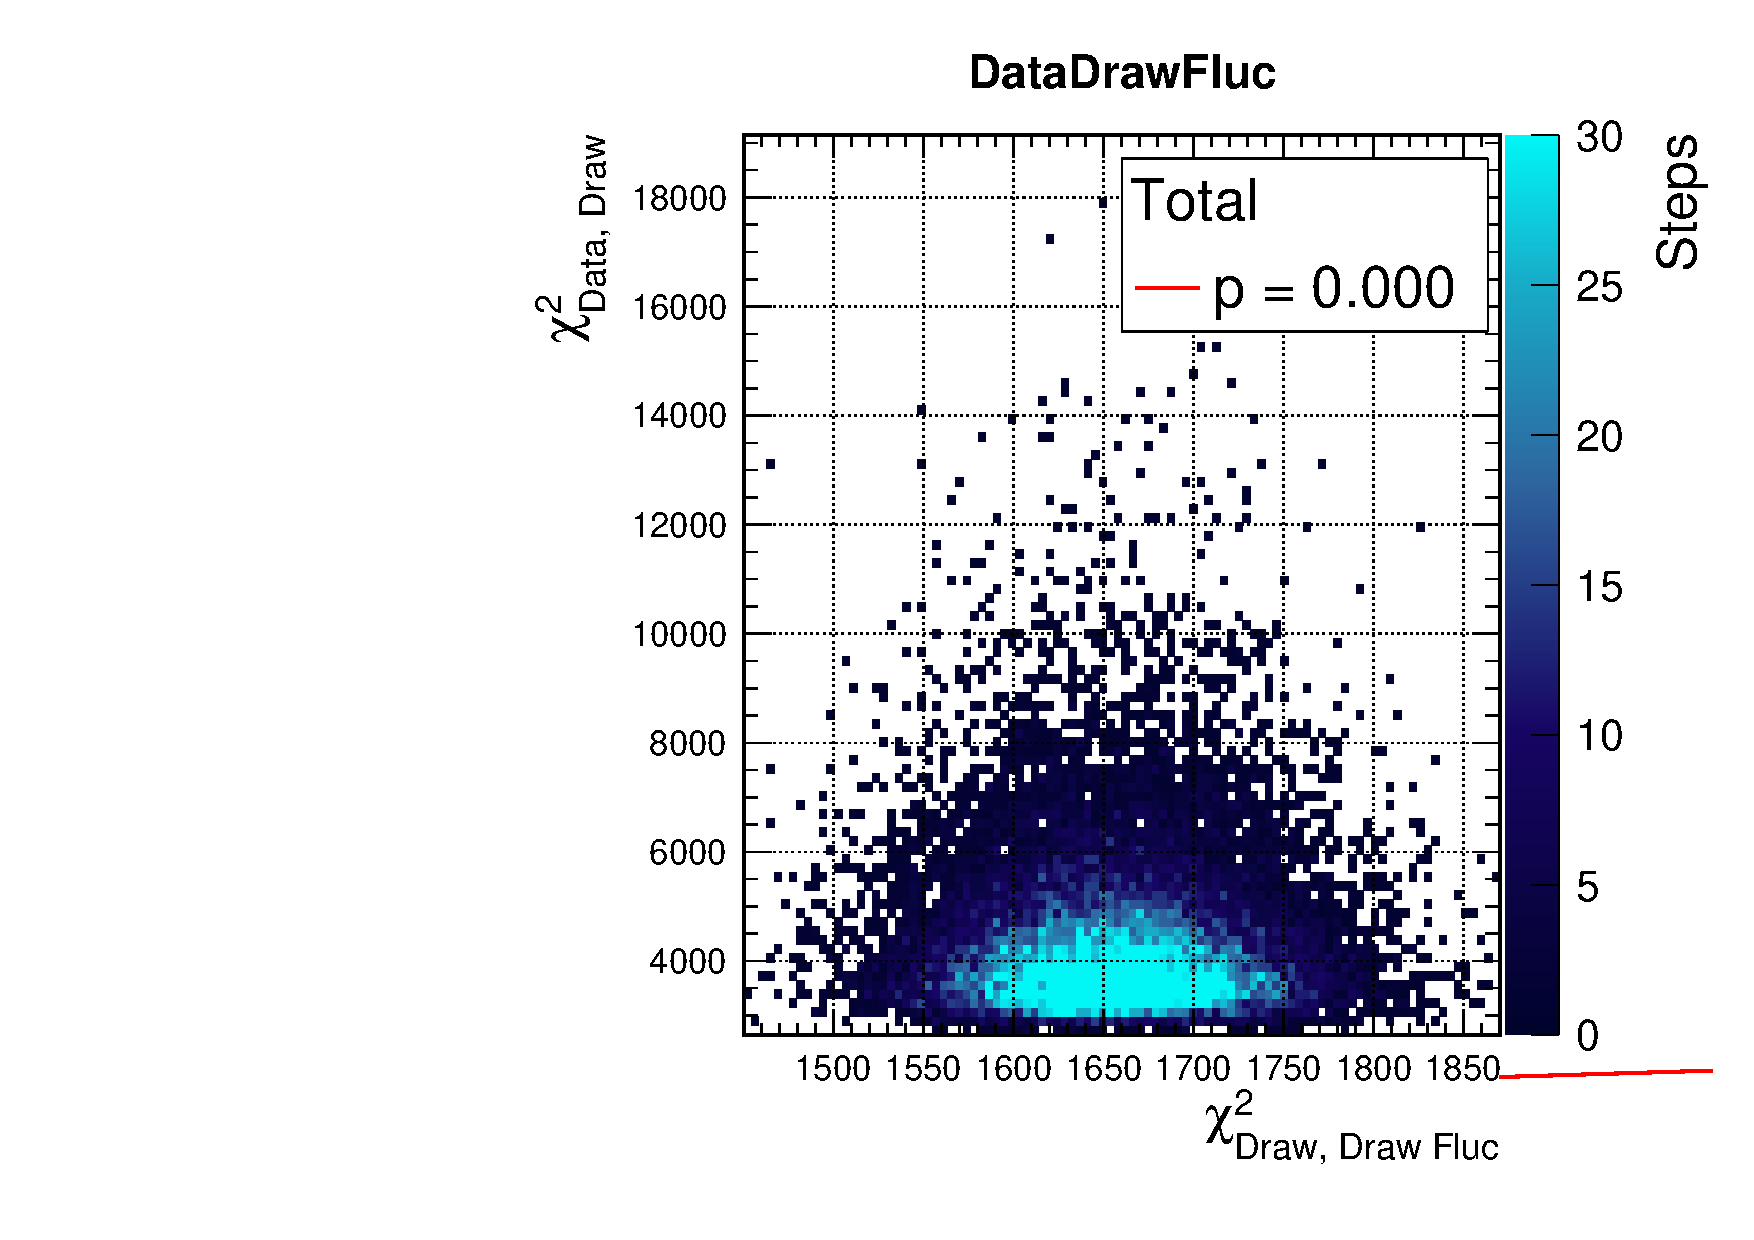
\includegraphics[width=\textwidth, trim={0mm 0mm 0mm 11mm}, clip,page=1]{figures/mach3/data/priorpred/2017b_NewDet_3Xsec_4Det_5Flux_NewXSecTune_Data_merge_PriorPred_procs}
	\end{subfigure}
	\begin{subfigure}[t]{0.49\textwidth}
		\includegraphics[width=\textwidth, trim={0mm 0mm 0mm 11mm}, clip,page=2]{figures/mach3/data/priorpred/2017b_NewDet_3Xsec_4Det_5Flux_NewXSecTune_Data_merge_PriorPred_procs}
	\end{subfigure}
	\caption{Prior predictive spectrum for the data fit}
	\label{fig:prior_pred_data}
\end{figure}

The table of prior predictive p-values broken down by sample is found in \autoref{tab:data_pre_pvalue}. The high-statistics FHC samples all consistently have $p=0.000$, and the low-statistics RHC samples have slightly higher p-values. This is primarily due to statistical fluctuations being a larger effect for the low-statistics samples compared to the size of the systematic fluctuations.
\begin{table}[h]
	\centering
	\begin{tabular}{l | c c }
		\hline \hline
		Sample & Draw Fluc. & Pred. Fluc. \\
		\hline
		FGD1 0$\pi$ & 0.000 & 0.000 \\
		FGD1 1$\pi$ & 0.000 & 0.000 \\
		FGD1 Other  & 0.000 & 0.000 \\
		\hline
		FGD2 0$\pi$ & 0.000 & 0.000 \\
		FGD2 1$\pi$ & 0.000 & 0.000 \\
		FGD2 Other  & 0.000 & 0.000 \\
		\hline
		FGD1 1Trk & 0.002 & 0.002 \\
		FGD1 NTrk & 0.003 & 0.002 \\
		FGD2 1Trk & 0.001 & 0.000 \\
		FGD2 NTrk & 0.017 & 0.017 \\
		\hline
		FGD1 \numu 1Trk & 0.004 & 0.004 \\
		FGD1 \numu NTrk & 0.011 & 0.009 \\
		FGD2 \numu 1Trk & 0.003 & 0.003 \\
		FGD2 \numu NTrk & 0.003 & 0.003 \\
		\hline
		\hline
	\end{tabular}
	\caption{Prior predictive p-values for each sample after the data fit}
	\label{tab:data_pre_pvalue}
\end{table}

\subsection{Posterior Predictive Spectrum}
\label{sec:post_pred_data}
The posterior predictive spectrum and p-values are calculated using the model after fitting to data. The resulting test-statistic distribution and p-value is shown in \autoref{fig:posterior_pred_data}, where $p = 0.000$\footnote{A rather discouraging result!}. 
\begin{figure}[h]
	\begin{subfigure}[t]{0.49\textwidth}
		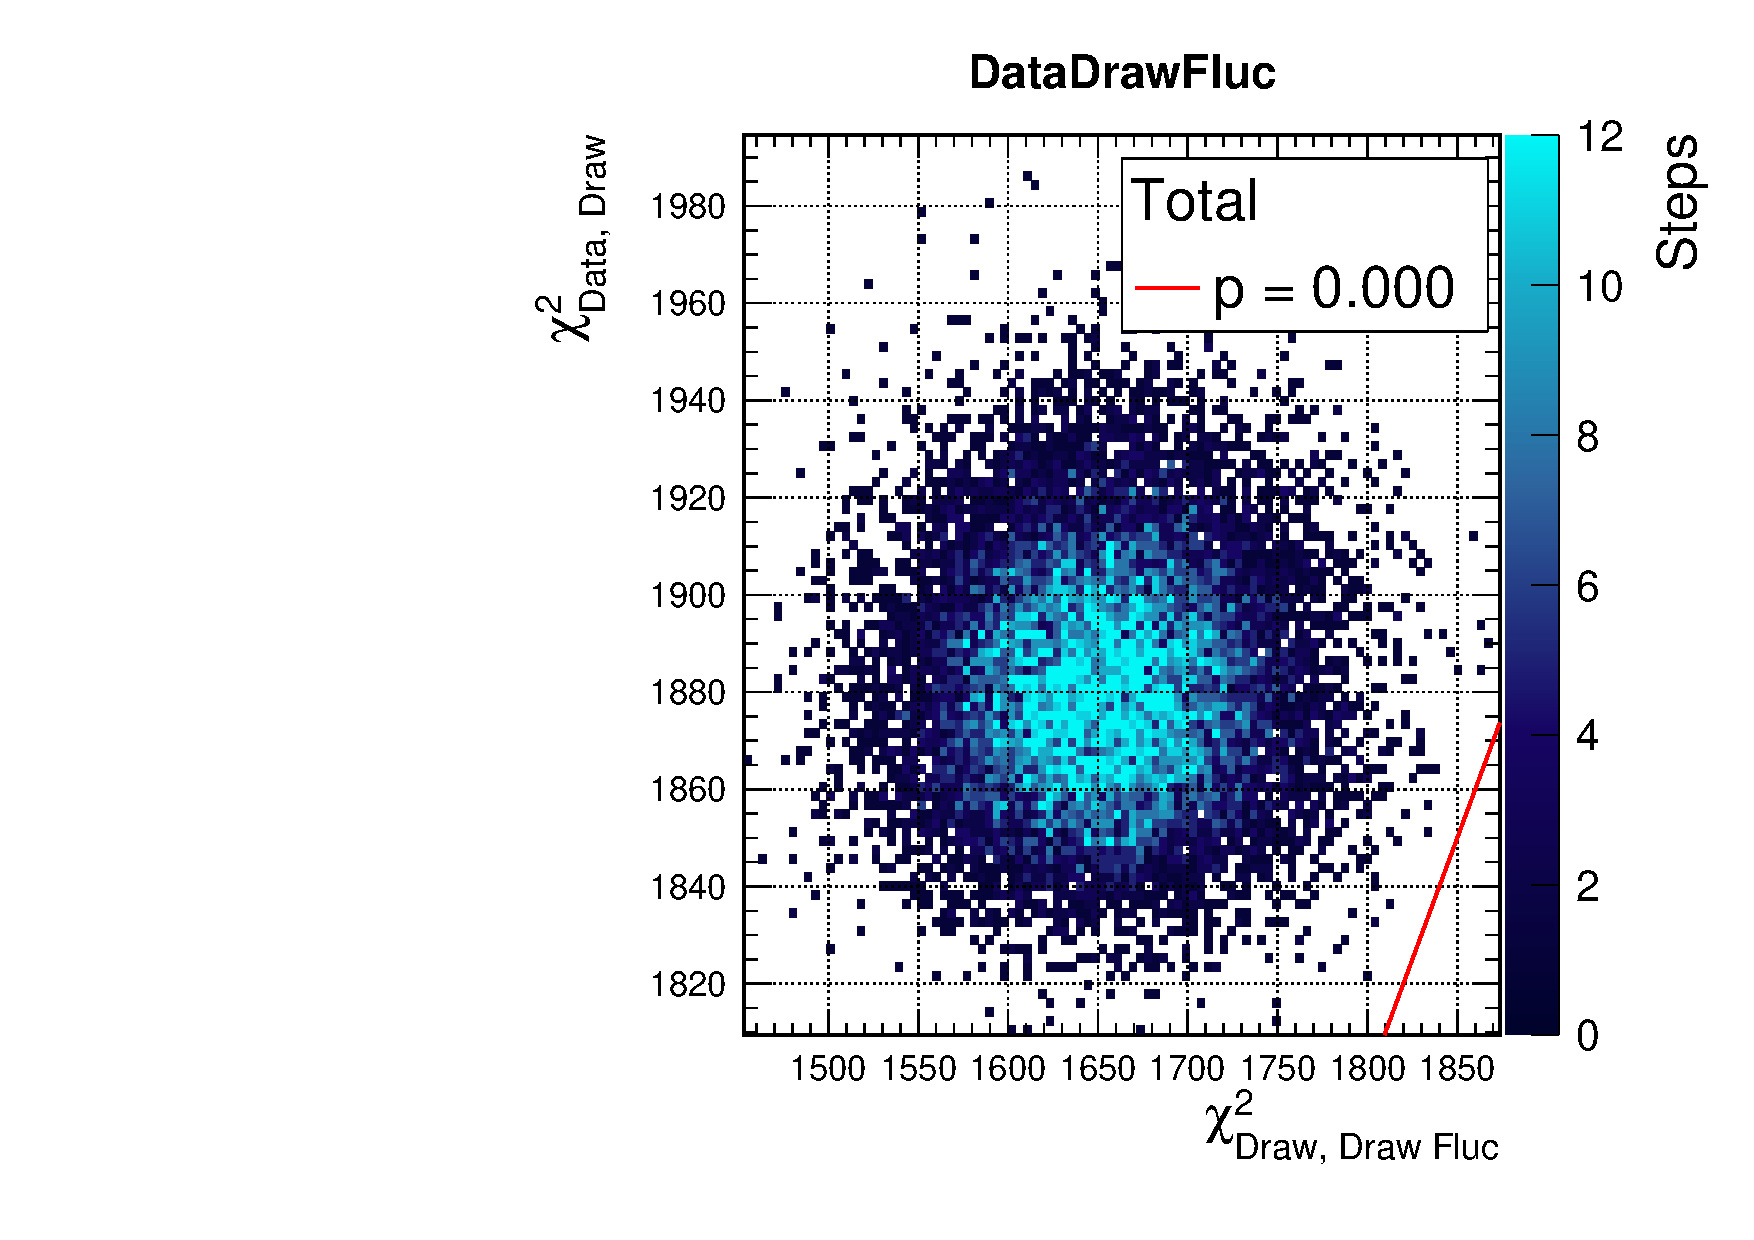
\includegraphics[width=\textwidth, trim={0mm 0mm 0mm 11mm}, clip,page=1]{figures/mach3/data/postpred/2017b_NewData_NewDet_UpdXsecStep_2Xsec_4Det_5Flux_0_PostPred_procs}
	\end{subfigure}
	\begin{subfigure}[t]{0.49\textwidth}
		\includegraphics[width=\textwidth, trim={0mm 0mm 0mm 11mm}, clip,page=2]{figures/mach3/data/postpred/2017b_NewData_NewDet_UpdXsecStep_2Xsec_4Det_5Flux_0_PostPred_procs}
	\end{subfigure}
	\caption{Posterior predictive spectrum for the data fit}
	\label{fig:posterior_pred_data}
\end{figure}

The p-values are broken down into sample contributions, and are presented in \autoref{tab:data_post_pvalue}. There are good p-values for all samples except FGD1 CCOther, which is zero. Importantly, the FGD2 CCOther selection observes a good p-value.
\begin{table}[h]
	\centering
\begin{tabular}{l | c c }
	\hline \hline
	Sample & Draw Fluc. & Pred. Fluc. \\
	\hline
	FGD1 0$\pi$ & 0.062 & 0.060 \\
	FGD1 1$\pi$ & 0.078 & 0.075 \\
	\textcolor{red}{FGD1 Other}  & \textcolor{red}{0.000} & \textcolor{red}{0.000} \\
	FGD2 0$\pi$ & 0.115 & 0.114 \\
	FGD2 1$\pi$ & 0.090 & 0.089 \\
	FGD2 Other  & 0.098 & 0.103 \\
	\hline
	FGD1 1Trk & 0.515 & 0.515 \\
	FGD1 NTrk & 0.292 & 0.289 \\
	FGD2 1Trk & 0.265 & 0.260 \\
	FGD2 NTrk & 0.230 & 0.219 \\
	\hline
	FGD1 \numu 1Trk & 0.296 & 0.293 \\
	FGD1 \numu NTrk & 0.842 & 0.839 \\
	FGD2 \numu 1Trk & 0.333 & 0.332 \\
	FGD2 \numu NTrk & 0.587 & 0.591 \\
	\hline
	\hline
\end{tabular}
\caption{Posterior predictive p-values for each sample after the data fit}
\label{tab:data_post_pvalue}
\end{table}

The test-statistic distributions for FGD1 CCOther are shown in \autoref{fig:posterior_pred_data_fgd1ccother} with FGD2 inset for comparison. Whereas the x-axes (statistically fluctuated test-statistic in the model) are similar for the two selections, we see a much higher test-statistic on the y-axis, reflecting the post-fit distribution is much less like the data for FGD1 than for FGD2. This was already hinted at in \autoref{tab:postfit_eventrate}, where FGD1 CCOther showed only a marginal improvement after the fit.
\begin{figure}[h]
	\begin{subfigure}[t]{0.49\textwidth}
		\includegraphics[width=\textwidth, trim={0mm 6mm 0mm 11mm}, clip,page=16]{figures/mach3/data/postpred/2017b_NewData_NewDet_UpdXsecStep_2Xsec_4Det_5Flux_0_PostPred_procs}
	\end{subfigure}
\begin{subfigure}[t]{0.49\textwidth}
	\includegraphics[width=\textwidth, trim={0mm 6mm 0mm 11mm}, clip,page=52]{figures/mach3/data/postpred/2017b_NewData_NewDet_UpdXsecStep_2Xsec_4Det_5Flux_0_PostPred_procs}
\end{subfigure}
	\caption{Bin-by-bin likelihood contributions in \pmu \cosmu for the CCOther selections}
	\label{fig:posterior_pred_data_fgd1ccother}
\end{figure}

\autoref{fig:posterior_pred_data_llh_ccother} shows the likelihood contribution per bin for FGD1 and FGD2 CCOther selections. As expected, there are more bins with high contributions for FGD1 than FGD2, especially at low $Q^2$, which are not present in FGD2. For FGD1 CCOther, the high likelihood contributions sit primarily at \cosmu=0.9-0.95, whereas FGD2 has its largest contributions scattered across the phase space.
\begin{figure}[h]
	\begin{subfigure}[t]{0.49\textwidth}
		\includegraphics[width=\textwidth, trim={0mm 6mm 0mm 11mm}, clip,page=21]{figures/mach3/data/postpred/2017b_NewData_NewDet_UpdXsecStep_2Xsec_4Det_5Flux_0_PostPred_procs}
		\caption{FGD1 CCOther}
	\end{subfigure}
	\begin{subfigure}[t]{0.49\textwidth}
		\includegraphics[width=\textwidth, trim={0mm 6mm 0mm 11mm}, clip,page=48]{figures/mach3/data/postpred/2017b_NewData_NewDet_UpdXsecStep_2Xsec_4Det_5Flux_0_PostPred_procs}
		\caption{FGD2 CCOther}
	\end{subfigure}
\caption{Posterior predictive p-values for the two CCOther selections after the data fit}
\label{fig:posterior_pred_data_llh_ccother}
\end{figure}

Inspecting the \pmu \cosmu post-fit distributions in \autoref{fig:postfit_pmucosmu_data_ccother}, the \pmu distributions appear different around 500-1000 MeV, where FGD2 sees a consistent underestimation and FGD1 instead looks statistically fluctuated, slightly above and under 1$\sigma$ from statistics. The CC DIS parameter is largely a normalisation up to 1.5 GeV. The distributions otherwise look very similar. The \cosmu projection of the two FGDs are consistent, with a mild difference at 0.8-0.92, where the bins show opposite behaviour, just outside 1$\sigma$. The CC DIS parameter has the smallest effect in the most forward-going bin.
\begin{figure}[h]
	\begin{subfigure}[t]{0.32\textwidth}
		\includegraphics[width=\textwidth,page=43,trim={0mm 125mm 40mm 0mm},clip]{{figures/mach3/selection/2017b_nominal_withdebug_forthesis_ND280_nom.pdf}}
	\end{subfigure}
	\begin{subfigure}[t]{0.32\textwidth}
		\includegraphics[width=\textwidth,page=43,trim={0mm 55mm 40mm 70mm},clip]{{figures/mach3/selection/2017b_nominal_withdebug_forthesis_ND280_nom.pdf}}
	\end{subfigure}
	\begin{subfigure}[t]{0.32\textwidth}
		\includegraphics[width=\textwidth,page=43,trim={0mm 0mm 40mm 140mm},clip]{{figures/mach3/selection/2017b_nominal_withdebug_forthesis_ND280_nom.pdf}}
	\end{subfigure}
	
	\begin{subfigure}[t]{\textwidth}
	\begin{subfigure}[t]{0.49\textwidth}
		\includegraphics[width=\textwidth, trim={0mm 0mm 0mm 6mm}, clip,page=101]{figures/mach3/data/postfit/2017b_NewDet_3Xsec_4Det_5Flux_NewXSecTune_Data_merge_PostFit_0_1_rootstack}
	\end{subfigure}
	\begin{subfigure}[t]{0.49\textwidth}
		\includegraphics[width=\textwidth, trim={0mm 0mm 0mm 6mm}, clip,page=102]{figures/mach3/data/postfit/2017b_NewDet_3Xsec_4Det_5Flux_NewXSecTune_Data_merge_PostFit_0_1_rootstack}
	\end{subfigure}
\caption{FGD1 CCOther}
\end{subfigure}
	
\begin{subfigure}[t]{\textwidth}
	\begin{subfigure}[t]{0.49\textwidth}
		\includegraphics[width=\textwidth, trim={0mm 0mm 0mm 6mm}, clip,page=223]{figures/mach3/data/postfit/2017b_NewDet_3Xsec_4Det_5Flux_NewXSecTune_Data_merge_PostFit_0_1_rootstack}
	\end{subfigure}
	\begin{subfigure}[t]{0.49\textwidth}
		\includegraphics[width=\textwidth, trim={0mm 0mm 0mm 6mm}, clip,page=224]{figures/mach3/data/postfit/2017b_NewDet_3Xsec_4Det_5Flux_NewXSecTune_Data_merge_PostFit_0_1_rootstack}
	\end{subfigure}
\caption{FGD2 CCOther}
\end{subfigure}
	\caption{Post-fit distributions for the CCOther selections in \pmu and \cosmu, showing the effect of the CC DIS parameter 1$\sigma$ variation}
	\label{fig:postfit_pmucosmu_data_ccother}
\end{figure}

Projecting the post-fit distributions onto $Q^2_{rec}$ and $E_\nu^{rec}$ in \autoref{fig:postfit_q2enu_data_ccother} the pattern becomes clearer: FGD1 has a consistent under-estimation in the $Q^2_{rec}=0.15-0.4\text{ GeV}^2$ range, whereas FGD2 has a good prediction in all but one bin. Additionally, the CC DIS parameter is almost entirely a normalisation parameter in $Q^2$, so the fit has little freedom from this parameter to change the $Q^2$ shape. Looking at the $E_\nu^{rec}$ distribution there is consistency across the two FGDs, although FGD1 is more underestimated in the 0.7-0.9 GeV range, approximately within 1$\sigma$ statistical uncertainty.
\begin{figure}[h]
	\begin{subfigure}[t]{0.32\textwidth}
		\includegraphics[width=\textwidth,page=43,trim={0mm 125mm 40mm 0mm},clip]{{figures/mach3/selection/2017b_nominal_withdebug_forthesis_ND280_nom.pdf}}
	\end{subfigure}
	\begin{subfigure}[t]{0.32\textwidth}
		\includegraphics[width=\textwidth,page=43,trim={0mm 55mm 40mm 70mm},clip]{{figures/mach3/selection/2017b_nominal_withdebug_forthesis_ND280_nom.pdf}}
	\end{subfigure}
	\begin{subfigure}[t]{0.32\textwidth}
		\includegraphics[width=\textwidth,page=43,trim={0mm 0mm 40mm 140mm},clip]{{figures/mach3/selection/2017b_nominal_withdebug_forthesis_ND280_nom.pdf}}
	\end{subfigure}

	\begin{subfigure}[t]{\textwidth}
	\begin{subfigure}[t]{0.49\textwidth}
		\includegraphics[width=\textwidth, trim={0mm 0mm 0mm 6mm}, clip,page=97]{figures/mach3/data/postfit/2017b_NewData_NewDet_UpdXsecStep_2Xsec_4Det_5Flux_0_PostFit_5_4_rootstack}
	\end{subfigure}
	\begin{subfigure}[t]{0.49\textwidth}
		\includegraphics[width=\textwidth, trim={0mm 0mm 0mm 6mm}, clip,page=98]{figures/mach3/data/postfit/2017b_NewData_NewDet_UpdXsecStep_2Xsec_4Det_5Flux_0_PostFit_5_4_rootstack}
	\end{subfigure}
\caption{FGD1 CCOther}
\end{subfigure}

\begin{subfigure}[t]{\textwidth}
\begin{subfigure}[t]{0.49\textwidth}
	\includegraphics[width=\textwidth, trim={0mm 0mm 0mm 6mm}, clip,page=219]{figures/mach3/data/postfit/2017b_NewData_NewDet_UpdXsecStep_2Xsec_4Det_5Flux_0_PostFit_5_4_rootstack}
\end{subfigure}
\begin{subfigure}[t]{0.49\textwidth}
	\includegraphics[width=\textwidth, trim={0mm 0mm 0mm 6mm}, clip,page=220]{figures/mach3/data/postfit/2017b_NewData_NewDet_UpdXsecStep_2Xsec_4Det_5Flux_0_PostFit_5_4_rootstack}
\end{subfigure}
\caption{FGD2 CCOther}
\end{subfigure}
	\caption{Post-fit distributions for the CCOther selections in $Q^2_{rec}$ and $E_\nu^{rec}$, showing the effect of the CC DIS parameter 1$\sigma$ variation}
	\label{fig:postfit_q2enu_data_ccother}
\end{figure}

The one-dimensional p-values are shown in \autoref{fig:posterior_pred_data_1d}, in which parameter sets from the posterior and prior probability distributions are taken as the reference distributions. The p-values are 10\% for both methods.
\begin{figure}[h]
	\begin{subfigure}[t]{0.49\textwidth}
		\includegraphics[width=\textwidth, trim={0mm 0mm 0mm 14mm}, clip,page=1]{figures/mach3/data/postpred/postpred_pvalue_1d}
		\caption{Posterior predictive, $p=0.10$}
	\end{subfigure}
	\begin{subfigure}[t]{0.49\textwidth}
		\includegraphics[width=\textwidth, trim={0mm 0mm 0mm 14mm}, clip,page=1]{figures/mach3/data/postpred/PriorPredictive_Hybrid}
		\caption{Prior predictive hybrid, $p=0.10$}
	\end{subfigure}
	\caption{One-dimensional p-value calculations, applying statistical fluctuations. The fraction above the red curve relative the total denotes the p-value. The red line is the realised p-value of the data-fit and the distribution is the statistically fluctuated reference distributions.}
	\label{fig:posterior_pred_data_1d}
\end{figure}

The two-dimensional p-values for the FGD1 CCOther selection in \autoref{tab:data_post_pvalue} were very poor, and the one-dimensional equivalent in \autoref{fig:posterior_pred_data_1d_ccother} concludes similarly. The realised test-statistic falls at the very end of the reference distribution.
\begin{figure}[h]
	\begin{subfigure}[t]{0.49\textwidth}
		\includegraphics[width=\textwidth, trim={0mm 0mm 0mm 14mm}, clip,page=1]{figures/mach3/data/postpred/pvalue_posteriorpred_fgd1ccother_1d}
		\caption{Posterior predictive, $p=0.00$}
	\end{subfigure}
	\begin{subfigure}[t]{0.49\textwidth}
		\includegraphics[width=\textwidth, trim={0mm 0mm 0mm 14mm}, clip,page=1]{figures/mach3/data/postpred/prior_pred_fgd1ccother}
		\caption{Prior predictive hybrid, $p=0.00$}
	\end{subfigure}
	\caption{One-dimensional p-value calculations for FGD1 CCOther}
	\label{fig:posterior_pred_data_1d_ccother}
\end{figure}

\subsection{Post-fit Distributions}
\autoref{fig:posterior_pred_data_fhc} and \autoref{fig:posterior_pred_data_rhc} shows all the selections' \pmu \cosmu distributions post-fit, using the posterior predictive spectrum as a representation of the post-fit Monte-Carlo. Clearly, the post-fit Monte-Carlo does not describe all distributions, and there are plenty of discrepancies in all selections. The 0$\pi$ and 1Trk selections generally see good predictions post-fit, especially around the flux peak. The 1$\pi$ and Other selections are patchier and it's difficult to spot patterns in $Q^2$, \pmu or \cosmu. Interestingly, the NTrk predictions are generally better than the 1$\pi$ and Other selections.
\begin{figure}[h]
	\begin{subfigure}[t]{0.32\textwidth}
		\includegraphics[width=\textwidth, trim={20mm 6mm 4mm 11mm}, clip,page=5]{figures/mach3/data/postpred/2017b_NewData_NewDet_UpdXsecStep_2Xsec_4Det_5Flux_0_PostPred_procs}
		\caption{FGD1 0$\pi$}
	\end{subfigure}
	\begin{subfigure}[t]{0.32\textwidth}
		\includegraphics[width=\textwidth, trim={20mm 6mm 4mm 11mm}, clip,page=14]{figures/mach3/data/postpred/2017b_NewData_NewDet_UpdXsecStep_2Xsec_4Det_5Flux_0_PostPred_procs}
		\caption{FGD1 1$\pi$}
	\end{subfigure}
	\begin{subfigure}[t]{0.32\textwidth}
		\includegraphics[width=\textwidth, trim={20mm 6mm 4mm 11mm}, clip,page=23]{figures/mach3/data/postpred/2017b_NewData_NewDet_UpdXsecStep_2Xsec_4Det_5Flux_0_PostPred_procs}
		\caption{FGD1 Other}
	\end{subfigure}

\begin{subfigure}[t]{0.32\textwidth}
	\includegraphics[width=\textwidth, trim={20mm 6mm 4mm 11mm}, clip,page=32]{figures/mach3/data/postpred/2017b_NewData_NewDet_UpdXsecStep_2Xsec_4Det_5Flux_0_PostPred_procs}
	\caption{FGD2 0$\pi$}
\end{subfigure}
\begin{subfigure}[t]{0.32\textwidth}
	\includegraphics[width=\textwidth, trim={20mm 6mm 4mm 11mm}, clip,page=41]{figures/mach3/data/postpred/2017b_NewData_NewDet_UpdXsecStep_2Xsec_4Det_5Flux_0_PostPred_procs}
	\caption{FGD2 1$\pi$}
\end{subfigure}
\begin{subfigure}[t]{0.32\textwidth}
	\includegraphics[width=\textwidth, trim={20mm 6mm 4mm 11mm}, clip,page=50]{figures/mach3/data/postpred/2017b_NewData_NewDet_UpdXsecStep_2Xsec_4Det_5Flux_0_PostPred_procs}
	\caption{FGD2 Other}
\end{subfigure}
\caption{Data to Posterior predictive \pmu \cosmu spectrum ratios after the fit for FHC selections}
\label{fig:posterior_pred_data_fhc}
\end{figure}

\begin{figure}[h]
\begin{subfigure}[t]{0.24\textwidth}
	\includegraphics[width=\textwidth, trim={20mm 6mm 4mm 11mm}, clip,page=59]{figures/mach3/data/postpred/2017b_NewData_NewDet_UpdXsecStep_2Xsec_4Det_5Flux_0_PostPred_procs}
	\caption{FGD1 1Trk}
\end{subfigure}
\begin{subfigure}[t]{0.24\textwidth}
	\includegraphics[width=\textwidth, trim={20mm 6mm 4mm 11mm}, clip,page=68]{figures/mach3/data/postpred/2017b_NewData_NewDet_UpdXsecStep_2Xsec_4Det_5Flux_0_PostPred_procs}
	\caption{FGD1 NTrk}
\end{subfigure}
\begin{subfigure}[t]{0.24\textwidth}
	\includegraphics[width=\textwidth, trim={20mm 6mm 4mm 11mm}, clip,page=77]{figures/mach3/data/postpred/2017b_NewData_NewDet_UpdXsecStep_2Xsec_4Det_5Flux_0_PostPred_procs}
	\caption{FGD2 1Trk}
\end{subfigure}
\begin{subfigure}[t]{0.24\textwidth}
\includegraphics[width=\textwidth, trim={20mm 6mm 4mm 11mm}, clip,page=86]{figures/mach3/data/postpred/2017b_NewData_NewDet_UpdXsecStep_2Xsec_4Det_5Flux_0_PostPred_procs}
\caption{FGD2 NTrk}
\end{subfigure}

\begin{subfigure}[t]{0.24\textwidth}
	\includegraphics[width=\textwidth, trim={20mm 6mm 4mm 11mm}, clip,page=95]{figures/mach3/data/postpred/2017b_NewData_NewDet_UpdXsecStep_2Xsec_4Det_5Flux_0_PostPred_procs}
	\caption{FGD1 \numu 1Trk}
\end{subfigure}
\begin{subfigure}[t]{0.24\textwidth}
	\includegraphics[width=\textwidth, trim={20mm 6mm 4mm 11mm}, clip,page=104]{figures/mach3/data/postpred/2017b_NewData_NewDet_UpdXsecStep_2Xsec_4Det_5Flux_0_PostPred_procs}
	\caption{FGD1 \numu NTrk}
\end{subfigure}
\begin{subfigure}[t]{0.24\textwidth}
	\includegraphics[width=\textwidth, trim={20mm 6mm 4mm 11mm}, clip,page=113]{figures/mach3/data/postpred/2017b_NewData_NewDet_UpdXsecStep_2Xsec_4Det_5Flux_0_PostPred_procs}
	\caption{FGD2 \numu 1Trk}
\end{subfigure}
\begin{subfigure}[t]{0.24\textwidth}
	\includegraphics[width=\textwidth, trim={20mm 6mm 4mm 11mm}, clip,page=122]{figures/mach3/data/postpred/2017b_NewData_NewDet_UpdXsecStep_2Xsec_4Det_5Flux_0_PostPred_procs}
	\caption{FGD1 \numu NTrk}
\end{subfigure}
\caption{Data to Posterior predictive \pmu \cosmu spectrum ratios after the fit for RHC selections}
\label{fig:posterior_pred_data_rhc}
\end{figure}

To better understand the effect of the fit the distributions are projected onto \pmu and \cosmu before and after the fit. \autoref{fig:fhc_postfit_0pi_1pi} shows the distributions using the prior and posterior predictive spectrum for FGD1 and 2 CC0$\pi$ and CC1$\pi$ selections. The uncertainties are evaluated using the full prior and posterior distributions.

For CC0$\pi$, there is some tension between FGD1 and FGD2 in the third \pmu bin for both the prior and posterior predictive distributions where the simulation describes FGD1 well but undershoots FGD2. The post-fit distribution instead fits FGD2 well in this bin and overestimates FGD1. There is good improvement in the first two \pmu bins in the post-fit and a large reduction in the overall error. Moving to the \cosmu distributions, there is little change in the central values, where the primary effect appears to be reducing the error band. In \cosmu there is good agreement between FGD1 and FGD2.

For CC1$\pi$, there is acceptable description in \pmu before the fit except in the first bin. In the 500-1000 MeV region there is consistent over-estimation of the events which gets mostly corrected in the fit. The highest bin is well described for FGD1 and less so for FGD2. The \cosmu distributions pre-fit distribution is much worse than \pmu, notably in the 0.8-0.98 region and especially present for FGD1. In the post-fit this is mostly corrected, although the 0.8-0.92 region is approximately 1$\sigma$ off.
\begin{figure}[h]
	\begin{subfigure}[t]{0.15\textwidth}
		\includegraphics[width=\textwidth, trim={0mm 90mm 0mm 0mm}, clip,page=1]{figures/mach3/1D_legend_Data_Posterior_Prior}
	\end{subfigure}
	\begin{subfigure}[t]{0.15\textwidth}
		\includegraphics[width=\textwidth, trim={0mm 45mm 0mm 50mm}, clip,page=1]{figures/mach3/1D_legend_Data_Posterior_Prior}
	\end{subfigure}	\begin{subfigure}[t]{0.15\textwidth}
	\includegraphics[width=\textwidth, trim={0mm 0mm 0mm 100mm}, clip,page=1]{figures/mach3/1D_legend_Data_Posterior_Prior}
\end{subfigure}
	
	\begin{subfigure}[t]{\textwidth}
	\begin{subfigure}[t]{0.24\textwidth}
		\includegraphics[width=\textwidth, trim={0mm 0mm 0mm 8mm}, clip,page=10]{figures/mach3/data/priorpred/2017b_NewDet_3Xsec_4Det_5Flux_NewXSecTune_Data_merge_PriorPred_procs}
	\end{subfigure}
	\begin{subfigure}[t]{0.24\textwidth}
		\includegraphics[width=\textwidth, trim={0mm 0mm 0mm 8mm}, clip,page=10]{figures/mach3/data/postpred/2017b_NewData_NewDet_UpdXsecStep_2Xsec_4Det_5Flux_0_PostPred_procs}
	\end{subfigure}
\begin{subfigure}[t]{0.24\textwidth}
\includegraphics[width=\textwidth, trim={0mm 0mm 0mm 8mm}, clip,page=11]{figures/mach3/data/priorpred/2017b_NewDet_3Xsec_4Det_5Flux_NewXSecTune_Data_merge_PriorPred_procs}
\end{subfigure}
	\begin{subfigure}[t]{0.24\textwidth}
		\includegraphics[width=\textwidth, trim={0mm 0mm 0mm 8mm}, clip,page=11]{figures/mach3/data/postpred/2017b_NewData_NewDet_UpdXsecStep_2Xsec_4Det_5Flux_0_PostPred_procs}
	\end{subfigure}
\caption{FGD1 0$\pi$}
\end{subfigure}
	
		\begin{subfigure}[t]{\textwidth}
	\begin{subfigure}[t]{0.24\textwidth}
		\includegraphics[width=\textwidth, trim={0mm 0mm 0mm 8mm}, clip,page=37]{figures/mach3/data/priorpred/2017b_NewDet_3Xsec_4Det_5Flux_NewXSecTune_Data_merge_PriorPred_procs}
	\end{subfigure}
	\begin{subfigure}[t]{0.24\textwidth}
		\includegraphics[width=\textwidth, trim={0mm 0mm 0mm 8mm}, clip,page=37]{figures/mach3/data/postpred/2017b_NewData_NewDet_UpdXsecStep_2Xsec_4Det_5Flux_0_PostPred_procs}
	\end{subfigure}
\begin{subfigure}[t]{0.24\textwidth}
\includegraphics[width=\textwidth, trim={0mm 0mm 0mm 8mm}, clip,page=38]{figures/mach3/data/priorpred/2017b_NewDet_3Xsec_4Det_5Flux_NewXSecTune_Data_merge_PriorPred_procs}
\end{subfigure}
	\begin{subfigure}[t]{0.24\textwidth}
		\includegraphics[width=\textwidth, trim={0mm 0mm 0mm 8mm}, clip,page=38]{figures/mach3/data/postpred/2017b_NewData_NewDet_UpdXsecStep_2Xsec_4Det_5Flux_0_PostPred_procs}
	\end{subfigure}
\caption{FGD2 0$\pi$}
\end{subfigure}
	
	\begin{subfigure}[t]{\textwidth}
	\begin{subfigure}[t]{0.24\textwidth}
		\includegraphics[width=\textwidth, trim={0mm 0mm 0mm 8mm}, clip,page=19]{figures/mach3/data/priorpred/2017b_NewDet_3Xsec_4Det_5Flux_NewXSecTune_Data_merge_PriorPred_procs}
	\end{subfigure}
	\begin{subfigure}[t]{0.24\textwidth}
		\includegraphics[width=\textwidth, trim={0mm 0mm 0mm 8mm}, clip,page=19]{figures/mach3/data/postpred/2017b_NewData_NewDet_UpdXsecStep_2Xsec_4Det_5Flux_0_PostPred_procs}
	\end{subfigure}
\begin{subfigure}[t]{0.24\textwidth}
\includegraphics[width=\textwidth, trim={0mm 0mm 0mm 8mm}, clip,page=20]{figures/mach3/data/priorpred/2017b_NewDet_3Xsec_4Det_5Flux_NewXSecTune_Data_merge_PriorPred_procs}
\end{subfigure}
	\begin{subfigure}[t]{0.24\textwidth}
		\includegraphics[width=\textwidth, trim={0mm 0mm 0mm 8mm}, clip,page=20]{figures/mach3/data/postpred/2017b_NewData_NewDet_UpdXsecStep_2Xsec_4Det_5Flux_0_PostPred_procs}
	\end{subfigure}
\caption{FGD1 1$\pi$}
\end{subfigure}

\begin{subfigure}[t]{\textwidth}
\begin{subfigure}[t]{0.24\textwidth}
	\includegraphics[width=\textwidth, trim={0mm 0mm 0mm 8mm}, clip,page=46]{figures/mach3/data/priorpred/2017b_NewDet_3Xsec_4Det_5Flux_NewXSecTune_Data_merge_PriorPred_procs}
\end{subfigure}
\begin{subfigure}[t]{0.24\textwidth}
	\includegraphics[width=\textwidth, trim={0mm 0mm 0mm 8mm}, clip,page=46]{figures/mach3/data/postpred/2017b_NewData_NewDet_UpdXsecStep_2Xsec_4Det_5Flux_0_PostPred_procs}
\end{subfigure}
\begin{subfigure}[t]{0.24\textwidth}
\includegraphics[width=\textwidth, trim={0mm 0mm 0mm 8mm}, clip,page=47]{figures/mach3/data/priorpred/2017b_NewDet_3Xsec_4Det_5Flux_NewXSecTune_Data_merge_PriorPred_procs}
\end{subfigure}
\begin{subfigure}[t]{0.24\textwidth}
	\includegraphics[width=\textwidth, trim={0mm 0mm 0mm 8mm}, clip,page=47]{figures/mach3/data/postpred/2017b_NewData_NewDet_UpdXsecStep_2Xsec_4Det_5Flux_0_PostPred_procs}
\end{subfigure}
\caption{FGD2 1$\pi$}
\end{subfigure}
\caption{FHC selections \pmu and \cosmu projections before and after fit}
\label{fig:fhc_postfit_0pi_1pi}
\end{figure}

\autoref{fig:fhc_postfit_other} shows the projections for FGD1 and FGD2 CCOther before and after the fit. The \pmu distributions are consistent between FGD1 and FGD2, which is underestimated around the maximum. The fit attempts to correct for this but it often settles somewhere in between the two. The \cosmu distributions are good up until \cosmu=0.85, where the prefit starts to underestimate the data. This underestimation is present after the fit too, and it appears the freedom in \cosmu is not sufficient to cover the data. 
\begin{figure}[h]
	\begin{subfigure}[t]{0.15\textwidth}
		\includegraphics[width=\textwidth, trim={0mm 90mm 0mm 0mm}, clip,page=1]{figures/mach3/1D_legend_Data_Posterior_Prior}
	\end{subfigure}
	\begin{subfigure}[t]{0.15\textwidth}
		\includegraphics[width=\textwidth, trim={0mm 45mm 0mm 50mm}, clip,page=1]{figures/mach3/1D_legend_Data_Posterior_Prior}
	\end{subfigure}	\begin{subfigure}[t]{0.15\textwidth}
		\includegraphics[width=\textwidth, trim={0mm 0mm 0mm 100mm}, clip,page=1]{figures/mach3/1D_legend_Data_Posterior_Prior}
	\end{subfigure}

\begin{subfigure}[t]{\textwidth}
\begin{subfigure}[t]{0.24\textwidth}
	\includegraphics[width=\textwidth, trim={0mm 0mm 0mm 8mm}, clip,page=28]{figures/mach3/data/priorpred/2017b_NewDet_3Xsec_4Det_5Flux_NewXSecTune_Data_merge_PriorPred_procs}
\end{subfigure}
\begin{subfigure}[t]{0.24\textwidth}
	\includegraphics[width=\textwidth, trim={0mm 0mm 0mm 8mm}, clip,page=28]{figures/mach3/data/postpred/2017b_NewData_NewDet_UpdXsecStep_2Xsec_4Det_5Flux_0_PostPred_procs}
\end{subfigure}
\begin{subfigure}[t]{0.24\textwidth}
\includegraphics[width=\textwidth, trim={0mm 0mm 0mm 8mm}, clip,page=29]{figures/mach3/data/priorpred/2017b_NewDet_3Xsec_4Det_5Flux_NewXSecTune_Data_merge_PriorPred_procs}
\end{subfigure}
\begin{subfigure}[t]{0.24\textwidth}
	\includegraphics[width=\textwidth, trim={0mm 0mm 0mm 8mm}, clip,page=29]{figures/mach3/data/postpred/2017b_NewData_NewDet_UpdXsecStep_2Xsec_4Det_5Flux_0_PostPred_procs}
\end{subfigure}
\caption{FGD1 Other}
\end{subfigure}

\begin{subfigure}[t]{\textwidth}
\begin{subfigure}[t]{0.24\textwidth}
	\includegraphics[width=\textwidth, trim={0mm 0mm 0mm 8mm}, clip,page=55]{figures/mach3/data/priorpred/2017b_NewDet_3Xsec_4Det_5Flux_NewXSecTune_Data_merge_PriorPred_procs}
\end{subfigure}
\begin{subfigure}[t]{0.24\textwidth}
	\includegraphics[width=\textwidth, trim={0mm 0mm 0mm 8mm}, clip,page=55]{figures/mach3/data/postpred/2017b_NewData_NewDet_UpdXsecStep_2Xsec_4Det_5Flux_0_PostPred_procs}
\end{subfigure}
\begin{subfigure}[t]{0.24\textwidth}
\includegraphics[width=\textwidth, trim={0mm 0mm 0mm 8mm}, clip,page=56]{figures/mach3/data/priorpred/2017b_NewDet_3Xsec_4Det_5Flux_NewXSecTune_Data_merge_PriorPred_procs}
\end{subfigure}
\begin{subfigure}[t]{0.24\textwidth}
	\includegraphics[width=\textwidth, trim={0mm 0mm 0mm 8mm}, clip,page=56]{figures/mach3/data/postpred/2017b_NewData_NewDet_UpdXsecStep_2Xsec_4Det_5Flux_0_PostPred_procs}
\end{subfigure}
\caption{FGD2 Other}
\end{subfigure}
\caption{FHC selections \pmu and \cosmu projections before and after fit}
\label{fig:fhc_postfit_other}
\end{figure}

\autoref{fig:rhc_postfit} shows the RHC \numubar selections for FGD1 and FGD2. For CC1Trk there are differences between FGD1 and FGD2 in the highest bin (around 400MeV), which the simulation describes well for FGD2 but not FGD1. Generally the pre-fit is adequate and the post-fit mostly reduces the error band. The largest difference is around 700 MeV for FGD2, which is well described for FGD1. For the \cosmu distributions, the pre-fit overestimates FGD1 but estimates FGD2 well. The post-fit instead under-estimates FGD2 slightly and estimates FGD1 well.

For the CCNTrk distributions the uncertainty from statistics are similar in error to the systematics and the prediction is generally good in \pmu pre-fit and post-fit; again the primary effect of the fit is to reduce the error rather than moving the central value. The \cosmu distribution is similarly well described pre-fit, although the second highest \cosmu bin is overestimated in FGD1 and the highest \cosmu bin is overestimated in FGD2. Post-fit, FGD1 is well described but FGD2 appears consistently over-estimated above \cosmu= 0.96, and the highest \cosmu bin is poorly described.
\begin{figure}[h]
	\begin{subfigure}[t]{0.15\textwidth}
		\includegraphics[width=\textwidth, trim={0mm 90mm 0mm 0mm}, clip,page=1]{figures/mach3/1D_legend_Data_Posterior_Prior}
	\end{subfigure}
	\begin{subfigure}[t]{0.15\textwidth}
		\includegraphics[width=\textwidth, trim={0mm 45mm 0mm 50mm}, clip,page=1]{figures/mach3/1D_legend_Data_Posterior_Prior}
	\end{subfigure}	\begin{subfigure}[t]{0.15\textwidth}
		\includegraphics[width=\textwidth, trim={0mm 0mm 0mm 100mm}, clip,page=1]{figures/mach3/1D_legend_Data_Posterior_Prior}
	\end{subfigure}

	\begin{subfigure}[t]{\textwidth}
	\begin{subfigure}[t]{0.24\textwidth}
		\includegraphics[width=\textwidth, trim={0mm 0mm 0mm 8mm}, clip,page=64]{figures/mach3/data/priorpred/2017b_NewDet_3Xsec_4Det_5Flux_NewXSecTune_Data_merge_PriorPred_procs}
	\end{subfigure}
	\begin{subfigure}[t]{0.24\textwidth}
		\includegraphics[width=\textwidth, trim={0mm 0mm 0mm 8mm}, clip,page=64]{figures/mach3/data/postpred/2017b_NewData_NewDet_UpdXsecStep_2Xsec_4Det_5Flux_0_PostPred_procs}
	\end{subfigure}
\begin{subfigure}[t]{0.24\textwidth}
\includegraphics[width=\textwidth, trim={0mm 0mm 0mm 8mm}, clip,page=65]{figures/mach3/data/priorpred/2017b_NewDet_3Xsec_4Det_5Flux_NewXSecTune_Data_merge_PriorPred_procs}
\end{subfigure}
	\begin{subfigure}[t]{0.24\textwidth}
		\includegraphics[width=\textwidth, trim={0mm 0mm 0mm 8mm}, clip,page=65]{figures/mach3/data/postpred/2017b_NewData_NewDet_UpdXsecStep_2Xsec_4Det_5Flux_0_PostPred_procs}
	\end{subfigure}
\caption{FGD1 1Trk}
\end{subfigure}
	
\begin{subfigure}[t]{\textwidth}
	\begin{subfigure}[t]{0.24\textwidth}
		\includegraphics[width=\textwidth, trim={0mm 0mm 0mm 8mm}, clip,page=82]{figures/mach3/data/priorpred/2017b_NewDet_3Xsec_4Det_5Flux_NewXSecTune_Data_merge_PriorPred_procs}
	\end{subfigure}
	\begin{subfigure}[t]{0.24\textwidth}
		\includegraphics[width=\textwidth, trim={0mm 0mm 0mm 8mm}, clip,page=82]{figures/mach3/data/postpred/2017b_NewData_NewDet_UpdXsecStep_2Xsec_4Det_5Flux_0_PostPred_procs}
	\end{subfigure}
\begin{subfigure}[t]{0.24\textwidth}
\includegraphics[width=\textwidth, trim={0mm 0mm 0mm 8mm}, clip,page=83]{figures/mach3/data/priorpred/2017b_NewDet_3Xsec_4Det_5Flux_NewXSecTune_Data_merge_PriorPred_procs}
\end{subfigure}
	\begin{subfigure}[t]{0.24\textwidth}
		\includegraphics[width=\textwidth, trim={0mm 0mm 0mm 8mm}, clip,page=83]{figures/mach3/data/postpred/2017b_NewData_NewDet_UpdXsecStep_2Xsec_4Det_5Flux_0_PostPred_procs}
	\end{subfigure}
\caption{FGD2 1Trk}
\end{subfigure}
	
\begin{subfigure}[t]{\textwidth}
	\begin{subfigure}[t]{0.24\textwidth}
		\includegraphics[width=\textwidth, trim={0mm 0mm 0mm 8mm}, clip,page=73]{figures/mach3/data/priorpred/2017b_NewDet_3Xsec_4Det_5Flux_NewXSecTune_Data_merge_PriorPred_procs}
	\end{subfigure}
	\begin{subfigure}[t]{0.24\textwidth}
		\includegraphics[width=\textwidth, trim={0mm 0mm 0mm 8mm}, clip,page=73]{figures/mach3/data/postpred/2017b_NewData_NewDet_UpdXsecStep_2Xsec_4Det_5Flux_0_PostPred_procs}
	\end{subfigure}
\begin{subfigure}[t]{0.24\textwidth}
\includegraphics[width=\textwidth, trim={0mm 0mm 0mm 8mm}, clip,page=74]{figures/mach3/data/priorpred/2017b_NewDet_3Xsec_4Det_5Flux_NewXSecTune_Data_merge_PriorPred_procs}
\end{subfigure}
	\begin{subfigure}[t]{0.24\textwidth}
		\includegraphics[width=\textwidth, trim={0mm 0mm 0mm 8mm}, clip,page=74]{figures/mach3/data/postpred/2017b_NewData_NewDet_UpdXsecStep_2Xsec_4Det_5Flux_0_PostPred_procs}
	\end{subfigure}
\caption{FGD1 NTrk}
\end{subfigure}

\begin{subfigure}[t]{\textwidth}
\begin{subfigure}[t]{0.24\textwidth}
	\includegraphics[width=\textwidth, trim={0mm 0mm 0mm 8mm}, clip,page=91]{figures/mach3/data/priorpred/2017b_NewDet_3Xsec_4Det_5Flux_NewXSecTune_Data_merge_PriorPred_procs}
\end{subfigure}
	\begin{subfigure}[t]{0.24\textwidth}
		\includegraphics[width=\textwidth, trim={0mm 0mm 0mm 8mm}, clip,page=91]{figures/mach3/data/postpred/2017b_NewData_NewDet_UpdXsecStep_2Xsec_4Det_5Flux_0_PostPred_procs}
	\end{subfigure}
\begin{subfigure}[t]{0.24\textwidth}
\includegraphics[width=\textwidth, trim={0mm 0mm 0mm 8mm}, clip,page=92]{figures/mach3/data/priorpred/2017b_NewDet_3Xsec_4Det_5Flux_NewXSecTune_Data_merge_PriorPred_procs}
\end{subfigure}
\begin{subfigure}[t]{0.24\textwidth}
\includegraphics[width=\textwidth, trim={0mm 0mm 0mm 8mm}, clip,page=92]{figures/mach3/data/postpred/2017b_NewData_NewDet_UpdXsecStep_2Xsec_4Det_5Flux_0_PostPred_procs}
\end{subfigure}
\caption{FGD2 NTrk}
\end{subfigure}
\caption{RHC \numubar selections \pmu and \cosmu projections before and after fit}
\label{fig:rhc_postfit}
\end{figure}

\autoref{fig:rhc_nu_postfit} shows FGD1 and FGD2 RHC \numu selections, which have comparably low statistics. The 1Trk distributions show consistency for FGD1 and FGD2. The only large discrepancy is found in the second last \cosmu bin for FGD1 and the last \cosmu bin for FGD2. The post-fit fails to correct for this and in general the fit minimises the error band rather than correcting the central values.

The NTrk distributions tell a similar story: the \pmu distributions are well-described by the prior model and are mildly improved by the post-fit model. For the \cosmu distribution the most forward-going bins are problematic for both FGD1 and FGD2, which the simulation underestimates.
\begin{figure}[h]
	\begin{subfigure}[t]{0.15\textwidth}
		\includegraphics[width=\textwidth, trim={0mm 90mm 0mm 0mm}, clip,page=1]{figures/mach3/1D_legend_Data_Posterior_Prior}
	\end{subfigure}
	\begin{subfigure}[t]{0.15\textwidth}
		\includegraphics[width=\textwidth, trim={0mm 45mm 0mm 50mm}, clip,page=1]{figures/mach3/1D_legend_Data_Posterior_Prior}
	\end{subfigure}	\begin{subfigure}[t]{0.15\textwidth}
		\includegraphics[width=\textwidth, trim={0mm 0mm 0mm 100mm}, clip,page=1]{figures/mach3/1D_legend_Data_Posterior_Prior}
	\end{subfigure}

	\begin{subfigure}[t]{\textwidth}
	\begin{subfigure}[t]{0.24\textwidth}
		\includegraphics[width=\textwidth, trim={0mm 0mm 0mm 8mm}, clip,page=100]{figures/mach3/data/priorpred/2017b_NewDet_3Xsec_4Det_5Flux_NewXSecTune_Data_merge_PriorPred_procs}
	\end{subfigure}
	\begin{subfigure}[t]{0.24\textwidth}
		\includegraphics[width=\textwidth, trim={0mm 0mm 0mm 8mm}, clip,page=100]{figures/mach3/data/postpred/2017b_NewData_NewDet_UpdXsecStep_2Xsec_4Det_5Flux_0_PostPred_procs}
	\end{subfigure}
\begin{subfigure}[t]{0.24\textwidth}
\includegraphics[width=\textwidth, trim={0mm 0mm 0mm 8mm}, clip,page=101]{figures/mach3/data/priorpred/2017b_NewDet_3Xsec_4Det_5Flux_NewXSecTune_Data_merge_PriorPred_procs}
\end{subfigure}
	\begin{subfigure}[t]{0.24\textwidth}
		\includegraphics[width=\textwidth, trim={0mm 0mm 0mm 8mm}, clip,page=101]{figures/mach3/data/postpred/2017b_NewData_NewDet_UpdXsecStep_2Xsec_4Det_5Flux_0_PostPred_procs}
	\end{subfigure}
\caption{FGD1 1Trk \numubar}
\end{subfigure}

\begin{subfigure}[t]{\textwidth}
\begin{subfigure}[t]{0.24\textwidth}
	\includegraphics[width=\textwidth, trim={0mm 0mm 0mm 8mm}, clip,page=118]{figures/mach3/data/priorpred/2017b_NewDet_3Xsec_4Det_5Flux_NewXSecTune_Data_merge_PriorPred_procs}
\end{subfigure}
	\begin{subfigure}[t]{0.24\textwidth}
	\includegraphics[width=\textwidth, trim={0mm 0mm 0mm 8mm}, clip,page=118]{figures/mach3/data/postpred/2017b_NewData_NewDet_UpdXsecStep_2Xsec_4Det_5Flux_0_PostPred_procs}
\end{subfigure}
\begin{subfigure}[t]{0.24\textwidth}
\includegraphics[width=\textwidth, trim={0mm 0mm 0mm 8mm}, clip,page=119]{figures/mach3/data/priorpred/2017b_NewDet_3Xsec_4Det_5Flux_NewXSecTune_Data_merge_PriorPred_procs}
\end{subfigure}
\begin{subfigure}[t]{0.24\textwidth}
	\includegraphics[width=\textwidth, trim={0mm 0mm 0mm 8mm}, clip,page=119]{figures/mach3/data/postpred/2017b_NewData_NewDet_UpdXsecStep_2Xsec_4Det_5Flux_0_PostPred_procs}
\end{subfigure}
\caption{FGD2 1Trk \numubar}
\end{subfigure}

\begin{subfigure}[t]{\textwidth}
\begin{subfigure}[t]{0.24\textwidth}
	\includegraphics[width=\textwidth, trim={0mm 0mm 0mm 8mm}, clip,page=109]{figures/mach3/data/priorpred/2017b_NewDet_3Xsec_4Det_5Flux_NewXSecTune_Data_merge_PriorPred_procs}
\end{subfigure}
\begin{subfigure}[t]{0.24\textwidth}
	\includegraphics[width=\textwidth, trim={0mm 0mm 0mm 8mm}, clip,page=109]{figures/mach3/data/postpred/2017b_NewData_NewDet_UpdXsecStep_2Xsec_4Det_5Flux_0_PostPred_procs}
\end{subfigure}
\begin{subfigure}[t]{0.24\textwidth}
\includegraphics[width=\textwidth, trim={0mm 0mm 0mm 8mm}, clip,page=110]{figures/mach3/data/priorpred/2017b_NewDet_3Xsec_4Det_5Flux_NewXSecTune_Data_merge_PriorPred_procs}
\end{subfigure}
\begin{subfigure}[t]{0.24\textwidth}
	\includegraphics[width=\textwidth, trim={0mm 0mm 0mm 8mm}, clip,page=110]{figures/mach3/data/postpred/2017b_NewData_NewDet_UpdXsecStep_2Xsec_4Det_5Flux_0_PostPred_procs}
\end{subfigure}
\caption{FGD1 NTrk \numubar}
\end{subfigure}

\begin{subfigure}[t]{\textwidth}
\begin{subfigure}[t]{0.24\textwidth}
	\includegraphics[width=\textwidth, trim={0mm 0mm 0mm 8mm}, clip,page=127]{figures/mach3/data/priorpred/2017b_NewDet_3Xsec_4Det_5Flux_NewXSecTune_Data_merge_PriorPred_procs}
\end{subfigure}
	\begin{subfigure}[t]{0.24\textwidth}
	\includegraphics[width=\textwidth, trim={0mm 0mm 0mm 8mm}, clip,page=127]{figures/mach3/data/postpred/2017b_NewData_NewDet_UpdXsecStep_2Xsec_4Det_5Flux_0_PostPred_procs}
\end{subfigure}
\begin{subfigure}[t]{0.24\textwidth}
\includegraphics[width=\textwidth, trim={0mm 0mm 0mm 8mm}, clip,page=128]{figures/mach3/data/priorpred/2017b_NewDet_3Xsec_4Det_5Flux_NewXSecTune_Data_merge_PriorPred_procs}
\end{subfigure}
\begin{subfigure}[t]{0.24\textwidth}
	\includegraphics[width=\textwidth, trim={0mm 0mm 0mm 8mm}, clip,page=128]{figures/mach3/data/postpred/2017b_NewData_NewDet_UpdXsecStep_2Xsec_4Det_5Flux_0_PostPred_procs}
\end{subfigure}
\caption{FGD2 NTrk \numubar}
\end{subfigure}
	\caption{RHC \numu selections \pmu and \cosmu projections before and after fit}
	\label{fig:rhc_nu_postfit}
\end{figure}

\subsection{Covariance Matrix from the Data Fit}
\label{sec:covariance_data}
\autoref{fig:postfit_corr_nd280} shows the post-fit covariance matrix for the ND280 parameters, directly comparable to the Asimov covariance matrix in \autoref{fig:asimov_nd_corr}. The bottom row shows the absolute difference in each matrix multiplied by the sign of each matrix. Blue entries have flipped sign, whereas red entries have kept their sign. The flux parameters never flip signs and generally the covariance barely changes, and the correlation maximally changes by $\sim0.2$. The only parameters that swap signs are the cross-section parameters. Although sometimes strong in the correlation plot, looking at the covariance plot the flip happens to parameters with weak constraints.

For the cross-section parameters there are stronger correlations between 2p2h shape C and 2p2h norm $\nu$ with the flux parameters. Whereas the 2p2h normalisation correlates stronger, the 2p2h shape parameter swaps sign frequently. This may be a result of the parameter being pushed against the boundary in the data fit. Interestingly, 2p2h norm $\nu$ correlates very differently with BeRPA A: the sign is swapped and the strength changes. This is largely expected: BeRPA A is pulled far from the value in the Asimov fit, so is entirely possible to correlate differently.

Looking at the correlations, there are strong relations between $M_A^{QE}$, 2p2h normalisations, BeRPA A, BeRPA B, $C_5^A$, CC DIS, NC other and the flux parameters. $M_A^{QE}$ correlates strongly with BeRPA A, B and D as expected from their parametrisations\footnote{Both being approximately $Q^2$ shape variations for CCQE interactions}. The correlations with the flux parameters is due to ND280 data sitting in a relatively small $E_\nu, Q^2$ region, correlating heavily with $E_\nu$ normalisations up to 1 GeV, in turn correlating with the other flux parameters due to the internal flux parameter correlations. The 2p2h normalisations contribute a relatively large portion of the uncertainty on the CC0$\pi$ sample across $E_\nu$, giving rise to the correlation. For the same reason, the $C_5^A$ correlations enter due to the parameter controlling the normalisation of one of the interaction terms in the single pion model. Finally the CC DIS parameter is parametrised as $0.4/E_\nu$ for DIS events, so directly correlates to any other parameters that are dependent on $E_\nu$, such as the flux parameters.
\begin{figure}[h]
\begin{subfigure}[t]{\textwidth}
	\begin{subfigure}[t]{0.49\textwidth}
		\includegraphics[width=\textwidth, trim={0mm 0mm 0mm 0mm}, clip,page=5]{figures/mach3/data/corr/2017b_NewData_NewDet_UpdXsecStep_2Xsec_4Det_5Flux_0_drawCorr}
	\end{subfigure}
	\begin{subfigure}[t]{0.49\textwidth}
		\includegraphics[width=\textwidth, trim={0mm 0mm 0mm 0mm}, clip,page=6]{figures/mach3/data/corr/2017b_NewData_NewDet_UpdXsecStep_2Xsec_4Det_5Flux_0_drawCorr}
	\end{subfigure}
\caption{$\sqrt{V_{i,j}}$ and correlation matrices}
\end{subfigure}

\begin{subfigure}[t]{\textwidth}
	\begin{subfigure}[t]{0.49\textwidth}
		\includegraphics[width=\textwidth, trim={0mm 0mm 0mm 0mm}, clip,page=1]{figures/mach3/data/corr/data_asimov_corr_ratio}
	\end{subfigure}
	\begin{subfigure}[t]{0.49\textwidth}
		\includegraphics[width=\textwidth, trim={0mm 0mm 0mm 0mm}, clip,page=2]{figures/mach3/data/corr/data_asimov_corr_ratio}
	\end{subfigure}
	\caption{$\sqrt{V_{i,j}}$ and correlation matrices for Asimov and data}
\end{subfigure}
\caption{Post-fit covariance matrix for the data fit, showing ND280 related parameters}
\label{fig:postfit_corr_nd280}
\end{figure}

%\autoref{fig:postfit_corr_flux}
%\begin{figure}[h]
%	\begin{subfigure}[t]{0.49\textwidth}
%		\includegraphics[width=\textwidth, trim={0mm 0mm 0mm 0mm}, clip,page=8]{figures/mach3/data/corr/2017b_NewData_NewDet_UpdXsecStep_2Xsec_4Det_5Flux_0_drawCorr}
%	\end{subfigure}
%	\begin{subfigure}[t]{0.49\textwidth}
%		\includegraphics[width=\textwidth, trim={0mm 0mm 0mm 0mm}, clip,page=9]{figures/mach3/data/corr/2017b_NewData_NewDet_UpdXsecStep_2Xsec_4Det_5Flux_0_drawCorr}
%	\end{subfigure}
%	\caption{Post-fit covariance matrix for the data fit, showing the flux parameters}
%	\label{fig:postfit_corr_flux}
%\end{figure}


%\autoref{fig:postfit_corr_xsec}
%\begin{figure}[h]
%	\begin{subfigure}[t]{0.49\textwidth}
%		\includegraphics[width=\textwidth, trim={0mm 0mm 0mm 0mm}, clip,page=11]{figures/mach3/data/corr/2017b_NewData_NewDet_UpdXsecStep_2Xsec_4Det_5Flux_0_drawCorr}
%	\end{subfigure}
%	\begin{subfigure}[t]{0.49\textwidth}
%		\includegraphics[width=\textwidth, trim={0mm 0mm 0mm 0mm}, clip,page=12]{figures/mach3/data/corr/2017b_NewData_NewDet_UpdXsecStep_2Xsec_4Det_5Flux_0_drawCorr}
%	\end{subfigure}
%	\caption{Post-fit covariance matrix for the data fit, showing the interaction parameters}
%	\label{fig:postfit_corr_xsec}
%\end{figure}

\subsection{Alternate Model and Compatibility Studies}
A number of alternative studies were performed for the 2017 analysis, comparing subruns in data and MC, change of model parameters and their priors, investigating effects of removing runs, and comparing FGD1 and FGD2. The largest impact was found in the FHC versus RHC data fit, and the FGD1 vs FGD2 data fit, with some parameters outside the $1\sigma$ range of the full fit to data. The posteriors from these two fits---and a fit using a 2015-like model with BeRPA and 2p2h shape fixed---were propagated to SK and event spectra comparisons were made. Generally, there were negligible ($<1\sigma$) differences with little impact on oscillation analyses. These studies are found in \autoref{sec:data_alt_studies}.

\section{Cross-group Validations}
Comparisons were made to the frequentist ``BANFF'' group to further validate the implementation and results of the ND280-only fits. The validation saw differences to this analysis in all of the flux parameters, and some of the interaction parameters. All were due to marginalisation effects when providing the point estimates from the MCMC. The posterior predictive distributions from the MCMC compared to the ``best-fit'' distributions from the global minimum agreed well and the validation tests were passed satisfactorily. \autoref{chap:banff_valid} details this procedure and the results